 \documentclass[final,fmstyle]{./util/fpunathesis}

% paquetes recomendados
\usepackage{amsmath,amsthm}
\usepackage{textcomp}
\usepackage[T1]{fontenc}
\usepackage[spanish]{babel}
\usepackage[utf8]{inputenc}
\usepackage{csquotes}
\usepackage{enumerate}
%\usepackage{enumitem}
\usepackage[shortlabels]{enumitem} %para enum con letras
\usepackage{caption}
\usepackage{subcaption}
\usepackage[style=numeric, uniquename=full, sorting=none,backend=biber, natbib=true]{biblatex}
\usepackage{listings}
% para la lista de simbolos
\usepackage{array} %for vertical thick lines in tables
\usepackage{multirow} %multirow tables
\usepackage{nicefrac} %for fractions like 1/4
%\usepackage[table]{xcolor} %para colorear las tablas
\usepackage{makecell}
\usepackage{tabto}    
\usepackage{xcolor}
%referencias
\addbibresource{referencias.bib}
%se importan las configuraciones custmizdas realizadas.
%%%%
%%% Conjuto de funciones utilitarias
%%% autor: Maximiliano Báez
%%% fecha: 25/08/2014
%%%

\usepackage{tablefootnote} %para utilizar \footnote{}
\usepackage{amssymb}
\renewcommand{\thefootnote}{\arabic{footnote}}

%%Para la construcción de la lista de simbolos
% Macro for 'List of Symbols', 'List of Notations' etc...
\def\listofsymbols{
    \newpage
\chapter*{Lista de Símbolos\hfill}
\addcontentsline{toc}{chapter}{Lista de Símbolos}
\begin{tabbing}

%\textit{HM} \indent \textit{High-slot Mark}\\
%\textit{MS} \indent \textit{Maximon Slot Index} - Mayor Índice de Ranura\\
\color{white}Zero \=\color{white}One \=\color{white}Twoooooo \=\color{white}Thre\\

\textit{HM} \>\>\>\textit{High-slot Mark}.\\
\textit{\(HM_{max}\)} \>\>\> HM máximo.\\

\textit{\(Ent_{link}\)} \>\>\> Entropía del enlace.\\
\textit{\(Ent_{link-i}\)} \>\>\> Entropía del enlace \textit{i}. \\
\textit{\(Ent_{red}\)} \>\>\> Entropía de la red. \\
\textit{N} \>\>\> Cantidad de \textit{FS} en un enlace.\\
\textit{\(FS_{i}\)} \>\>\> \textit{Frecuency Slot} de índice \textit{i}.\\
\textit{\(FS_{i+1}\)} \>\>\> \textit{Frecuency Slot} de índice \(\textit{i} + 1\).\\
|\textit{E}| \>\>\> Cantidad de enlaces de la red.\\

\textit{\(SHF_{link}\)} \>\>\> Entropía de Shannon del enlace.\\
\textit{\(SHF_{link-i}\)} \>\>\> Entropía de Shannon del enlace \textit{i}. \\
\textit{\(SHF_{red}\)} \>\>\> Entropía de Shannon de la red. \\
\textit{\(S_{free}\)} \>\>\> Cantidad de \textit{FS} libres en un enlace.\\

\textit{\(BFR_{link}\)} \>\>\> Relación de Fragmentación de ancho de banda de un enlace.\\
\textit{\(BFR_{link-i}\)} \>\>\> Relación de Fragmentación de ancho de banda del enlace \textit{i}. \\
\textit{\(BFR_{red}\)} \>\>\> Relación de Fragmentación de ancho de banda de la red. \\
\textit{MaxBlock()} \>\>\> Tamaño del mayor bloque de \textit{FS} bloquados.\\

\textit{MSI} \>\>\> Índice de slot máximo utilizado.\\
\textit{\(MSI_{link-i}\)} \>\>\> Índice de slot máximo utilizado del enlace \textit{i}. \\
\textit{\(MSI_{red}\)} \>\>\> Índice de slot máximo utilizado de la red. \\

\textit{\(CE_{link}\)} \>\>\> Consecutividad del espectro.\\
\textit{\(CE_{red}\)} \>\>\> Consecutividad del espectro de la red. \\
\textit{Joins} \>\>\> Cantidad total de bloques de dos ranuras libres adyacentes\\ 
                \>\>\>  distintos dentro de un enlace.\\
\textit{Bloques} \>\>\> Cantidad de bloques de ranuras libres en un enlace. \\
\textit{K} \>\>\> Cantidad de rutas de dos enlaces en la red.\\

\textit{Uso} \>\>\> Porcentaje de utilización de la red.\\
\textit{sum(i)} \>\>\> Cantidad de \textit{FS} utilizadas en el enlace \textit{i}.\\

\textit{FSB} \>\>\> Acumulación de \textit{FS} bloqueados.\\
\textit{\(S_{i}^{block}\)} \>\>\> Cantidad de \textit{FS} solicitadas por la demanda bloqueada \textit{i}.\\
\textit{D} \>\>\> Cantidad de demandas.\\
\textit{T} \>\>\> Ventada de tiempo seleccionada para el calculo de \textit{IB}.\\

\textit{\(PB_{t}\)} \>\>\> Índice de bloqueo para el tiempo \textit{t}.\\
\textit{\(FSD_{i}\)} \>\>\> Cantidad de \textit{FS} demandadas en el tiempo \textit{t}.\\ 

\textit{\(train_{mean}\)} \>\>\> Media de valores.\\
\textit{\(train_{stf}\)} \>\>\> Desviación estándar.\\

\textit{MAE} \>\>\> Error Absoluto Medio.\\
\textit{MSE} \>\>\> Error Cuadrático Medio.\\

\textit{PB} \>\>\> Probabilidad de Bloqueo.\\
\textit{\(PB_{th}\)} \>\>\> Umbral para disparar el proceso de desfragmentación.\\

\textit{BL} \>\>\> Cantidad de Bloqueos.\\
\textit{RC} \>\>\> Cantidad de Reconfiguraciones.\\
\textit{SFP} \>\>\> Número de soluciones en el Frente Pareto.\\
\textit{CP} \>\>\> Cobertura Pareto.\\
\textit{MP} \>\>\> Método Propuesto.
% \begin{tabular}{p{0.1\linewidth}p{0.9\linewidth}}
% \textit{HM} & \textit{High-slot Mark} \\
% \textit{MS} & \textit{Maximun Slot Index} - Mayor Índice de Ranura \\
% \end{tabular}
\end{tabbing}

    \clearpage{}
}
\def\newsymbol #1: #2#3{$#1$ \> \parbox{5in}{#2 \dotfill \pageref{#3}}\\}
\def\addsymbol#1{\label{#1}}

% Para las imagenes en grilla
% custom commands
\newcommand{\foreign}[1]{{\it #1}}
\DeclareMathOperator*{\argmax}{arg\,max}
%\algsetup{}
\algsetup{
    indent=4em,
    linenosize=\small,
    linenodelimiter=.
}

\usepackage{amsmath}

%% se utilizan para referenciar figuras, tablas, secciones y algoritmos
\newcommand{\figref}[1]{Figura \ref{#1}}
\newcommand{\tabref}[1]{Tabla \ref{#1}}
\newcommand{\secref}[1]{sección \ref{#1}}
\newcommand{\algref}[1]{Algoritmo \ref{#1}}


%Traducción al español del paquete algorithmic%
\floatname{algorithm}{Algoritmo}
\renewcommand{\listalgorithmname}{Lista de algoritmos}
\renewcommand{\algorithmicrequire}{\textbf{Entrada:}}
\renewcommand{\algorithmicensure}{\textbf{Salida:}}
\renewcommand{\algorithmicend}{\textbf{fin}}
\renewcommand{\algorithmicif}{\textbf{si}}
\renewcommand{\algorithmicthen}{\textbf{entonces}}
\renewcommand{\algorithmicelse}{\textbf{si no}}
\renewcommand{\algorithmicelsif}{\algorithmicelse,\ \algorithmicif}
\renewcommand{\algorithmicendif}{\algorithmicend\ \algorithmicif}
\renewcommand{\algorithmicfor}{\textbf{para}}
\renewcommand{\algorithmicforall}{\textbf{para todo}}
\renewcommand{\algorithmicdo}{\textbf{hacer}}
\renewcommand{\algorithmicendfor}{\algorithmicend\ \algorithmicfor}
\renewcommand{\algorithmicwhile}{\textbf{mientras}}
\renewcommand{\algorithmicendwhile}{\algorithmicend\ \algorithmicwhile}
\renewcommand{\algorithmicloop}{\textbf{repetir}}
\renewcommand{\algorithmicendloop}{\algorithmicend\ \algorithmicloop}
\renewcommand{\algorithmicrepeat}{\textbf{repetir}}
\renewcommand{\algorithmicuntil}{\textbf{hasta que}}
\renewcommand{\algorithmicprint}{\textbf{imprimir}}
\renewcommand{\algorithmicreturn}{\textbf{retorna}}
\renewcommand{\algorithmictrue}{\textbf{cierto }}
\renewcommand{\algorithmicfalse}{\textbf{falso }}
\renewcommand{\algorithmiccomment}{\textbf{comentario : }}


% datos de la tesis y el/los autor/es
\title{Estrategia de disparo para el proceso de desfragmentación en redes ópticas elásticas multicore, utilizando técnicas de aprendizaje automático}
\author{RODOLFO SEBASTIÁN VERGARA FERREIRA \and DIEGO DANIEL DUARTE CENTURIÓN}
\degree{Informática}

\advisor{Phd. Msc. Ing.}{ENRIQUE DAVALOS}

%\newtheorem{definicion}{Definición}

\logosource{./graphics/logo.png}


\begin{document}
\renewcommand{\listtablename}{Lista de Tablas}
\renewcommand{\tablename}{Tabla}
\maketitle     % esto hace las portadas

% Agradecimientos
%\include{book/agradecimientos}

% los siguientes comandos producen 'indices.

% Tabla de contenidos
\tableofcontents
% Lista de figuras, incluye en la lista todas las figuras de forma automática
\listoffigures
% Lista de tablas, incluye en la lista todas las tablas de forma automática
\listoftables
% Lista de algoritmos, incluye en la lista todas los algoritmos de forma automática
%\listofalgorithms
%\include{acronimos}
\newpage
\chapter*{Lista de Símbolos\hfill}
\addcontentsline{toc}{chapter}{Lista de Símbolos}
\begin{tabbing}

%\textit{HM} \indent \textit{High-slot Mark}\\
%\textit{MS} \indent \textit{Maximon Slot Index} - Mayor Índice de Ranura\\
\color{white}Zero \=\color{white}One \=\color{white}Twoooooo \=\color{white}Thre\\

\textit{HM} \>\>\>\textit{High-slot Mark}.\\
\textit{\(HM_{max}\)} \>\>\> HM máximo.\\

\textit{\(Ent_{link}\)} \>\>\> Entropía del enlace.\\
\textit{\(Ent_{link-i}\)} \>\>\> Entropía del enlace \textit{i}. \\
\textit{\(Ent_{red}\)} \>\>\> Entropía de la red. \\
\textit{N} \>\>\> Cantidad de \textit{FS} en un enlace.\\
\textit{\(FS_{i}\)} \>\>\> \textit{Frecuency Slot} de índice \textit{i}.\\
\textit{\(FS_{i+1}\)} \>\>\> \textit{Frecuency Slot} de índice \(\textit{i} + 1\).\\
|\textit{E}| \>\>\> Cantidad de enlaces de la red.\\

\textit{\(SHF_{link}\)} \>\>\> Entropía de Shannon del enlace.\\
\textit{\(SHF_{link-i}\)} \>\>\> Entropía de Shannon del enlace \textit{i}. \\
\textit{\(SHF_{red}\)} \>\>\> Entropía de Shannon de la red. \\
\textit{\(S_{free}\)} \>\>\> Cantidad de \textit{FS} libres en un enlace.\\

\textit{\(BFR_{link}\)} \>\>\> Relación de Fragmentación de ancho de banda de un enlace.\\
\textit{\(BFR_{link-i}\)} \>\>\> Relación de Fragmentación de ancho de banda del enlace \textit{i}. \\
\textit{\(BFR_{red}\)} \>\>\> Relación de Fragmentación de ancho de banda de la red. \\
\textit{MaxBlock()} \>\>\> Tamaño del mayor bloque de \textit{FS} bloquados.\\

\textit{MSI} \>\>\> Índice de slot máximo utilizado.\\
\textit{\(MSI_{link-i}\)} \>\>\> Índice de slot máximo utilizado del enlace \textit{i}. \\
\textit{\(MSI_{red}\)} \>\>\> Índice de slot máximo utilizado de la red. \\

\textit{\(CE_{link}\)} \>\>\> Consecutividad del espectro.\\
\textit{\(CE_{red}\)} \>\>\> Consecutividad del espectro de la red. \\
\textit{Joins} \>\>\> Cantidad total de bloques de dos ranuras libres adyacentes\\ 
                \>\>\>  distintos dentro de un enlace.\\
\textit{Bloques} \>\>\> Cantidad de bloques de ranuras libres en un enlace. \\
\textit{K} \>\>\> Cantidad de rutas de dos enlaces en la red.\\

\textit{Uso} \>\>\> Porcentaje de utilización de la red.\\
\textit{sum(i)} \>\>\> Cantidad de \textit{FS} utilizadas en el enlace \textit{i}.\\

\textit{FSB} \>\>\> Acumulación de \textit{FS} bloqueados.\\
\textit{\(S_{i}^{block}\)} \>\>\> Cantidad de \textit{FS} solicitadas por la demanda bloqueada \textit{i}.\\
\textit{D} \>\>\> Cantidad de demandas.\\
\textit{T} \>\>\> Ventada de tiempo seleccionada para el calculo de \textit{IB}.\\

\textit{\(PB_{t}\)} \>\>\> Índice de bloqueo para el tiempo \textit{t}.\\
\textit{\(FSD_{i}\)} \>\>\> Cantidad de \textit{FS} demandadas en el tiempo \textit{t}.\\ 

\textit{\(train_{mean}\)} \>\>\> Media de valores.\\
\textit{\(train_{stf}\)} \>\>\> Desviación estándar.\\

\textit{MAE} \>\>\> Error Absoluto Medio.\\
\textit{MSE} \>\>\> Error Cuadrático Medio.\\

\textit{PB} \>\>\> Probabilidad de Bloqueo.\\
\textit{\(PB_{th}\)} \>\>\> Umbral para disparar el proceso de desfragmentación.\\

\textit{BL} \>\>\> Cantidad de Bloqueos.\\
\textit{RC} \>\>\> Cantidad de Reconfiguraciones.\\
\textit{SFP} \>\>\> Número de soluciones en el Frente Pareto.\\
\textit{CP} \>\>\> Cobertura Pareto.\\
\textit{MP} \>\>\> Método Propuesto.
% \begin{tabular}{p{0.1\linewidth}p{0.9\linewidth}}
% \textit{HM} & \textit{High-slot Mark} \\
% \textit{MS} & \textit{Maximun Slot Index} - Mayor Índice de Ranura \\
% \end{tabular}
\end{tabbing}



\mainmatter  % inician los capítulos de la tesis


% incluye aqui los capítulos (un archivo .tex por capitulo)
%\chapter{Capítulo de Ejemplo}

\section{Figuras, tablas y algoritmos}

\label{sec:figuras-tablas-algoritmos}
\subsection{Figuras}
Ejemplo de como hacer figuras utilizando el paquete figure\footnote{http://en.wikibooks.org/wiki/LaTeX/Floats,\_Figures\_and\_Captions} de LaTex.
\begin{figure}[!htbp]
    \centering
    
\includegraphics[width=0.5\textwidth]{capitulo-ej/graphics/latex.jpg}
    \caption{\label{fig:figura-ejemplo}Ejemplo de una figura en LaTex.}

\end{figure}

\begin{figure}[!htbp]
    \centering
    \begin{subfigure}[b]{0.45\textwidth}
            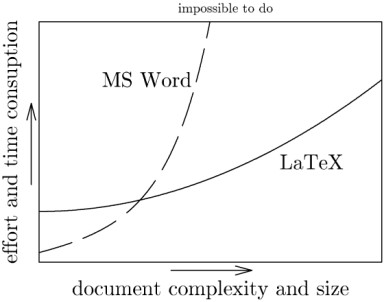
\includegraphics[width=\textwidth]{capitulo-ej/graphics/ejemplo-1.jpg}
            \caption{Subfigura 1.}
    \end{subfigure}
    ~~~~
    \begin{subfigure}[b]{0.45\textwidth}
            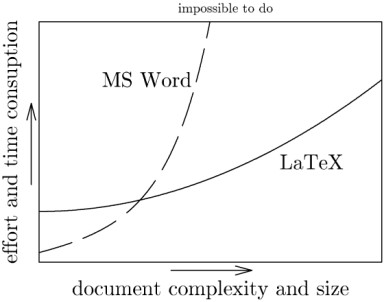
\includegraphics[width=\textwidth]{capitulo-ej/graphics/ejemplo-1.jpg}
            \caption{Subfigura 2.}

    \end{subfigure}
    \begin{subfigure}[b]{0.45\textwidth}
            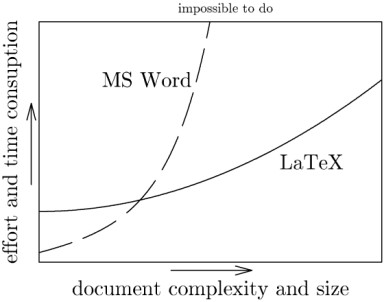
\includegraphics[width=\textwidth]{capitulo-ej/graphics/ejemplo-1.jpg}
            \caption{Subfigura 3.}
    \end{subfigure}
    ~~~~
    \begin{subfigure}[b]{0.45\textwidth}
            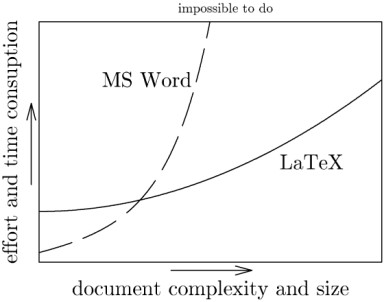
\includegraphics[width=\textwidth]{capitulo-ej/graphics/ejemplo-1.jpg}
            \caption{Subfigura 4.}

    \end{subfigure}
    \caption{\label{fig:ejemplo-fig-grilla}Ejemplo de una grilla de figuras en LaTex.}

\end{figure}

\subsection{Tablas}
Ejemplo de como hacer tablas utilizando el paquete table\footnote{http://en.wikibooks.org/wiki/LaTeX/Tables} de LaTex.
\begin{table}[!htpb]
    \begin{minipage}{\textwidth}
        \begin{center}
        \caption{\label{tab:tabla-ejemplo} Ejemplo de una tabla en LaTex.}
        \begin{tabular}{p{3cm} c c c c}
            \hline\\
            Año & Periodo & Columna & Columna2 & Columna3\\
            \hline
            \hline\\
            2014 & 29-12-13 / 31-05-14 & 10541 & 1052 & 2\\
            2013 & 30-12-12 / 21-12-13 & 153793 & 131306 & 70\\
            2012 & 01-01-12 / 22-12-12 & 37815 & 30588 & 11\\
            2011 & 03-01-11 / 29-12-11 & 53397 & 42264 & 62\\
            2010 & 11-10-09 / 25-12-10 & 21951 & 13760 & --$^a$\\
        \end{tabular}
        \footnotetext[1]{Esta es una nota.}
        \end{center}
    \end{minipage}
\end{table}

\subsection{Algoritmos}
Ejemplo de como hacer agloritmos utilizando el paquete algorithm\footnote{http://en.wikibooks.org/wiki/LaTeX/Algorithms} de LaTex.
\begin{algorithm}                      % enter the algorithm environment
\caption{Calculate $y = x^n$}          % give the algorithm a caption
\label{alg:alg1}                       % and a label for \ref{} commands later in the document
\begin{algorithmic}                    % enter the algorithmic environment
    \REQUIRE $n \geq 0 \vee x \neq 0$
    \ENSURE $y = x^n$
    \STATE $y \Leftarrow 1$
    \IF{$n < 0$}
        \STATE $X \Leftarrow 1 / x$
        \STATE $N \Leftarrow -n$
    \ELSE
        \STATE $X \Leftarrow x$
        \STATE $N \Leftarrow n$
    \ENDIF
    \WHILE{$N \neq 0$}
        \IF{$N$ is even}
            \STATE $X \Leftarrow X \times X$
            \STATE $N \Leftarrow N / 2$
        \ELSE[$N$ is odd]
            \STATE $y \Leftarrow y \times X$
            \STATE $N \Leftarrow N - 1$
        \ENDIF
    \ENDWHILE
\end{algorithmic}
\end{algorithm}

\subsection{Ecuaciones}
En esta sección se añade una pequeña ecuación con el fin de ejemplificar su
uso \addsymbol{symbol:x} \addsymbol{symbol:a_i}.
\begin{equation}\label{eq:ecuacion-ej}
  x = a_0 + \cfrac{1}{a_1
          + \cfrac{1}{a_2
          + \cfrac{1}{a_3 + \cfrac{1}{a_4} } } }
\end{equation}

\section{Referencias y citaciones}
Para referenciar secciones, figuras, tablas, algoritmos, o formulas se puede
emplear $\setminus$ref\{label-del-item\} o emplear cualquiera de las sigientes macros:


\begin{itemize}
\item $\setminus$secref\{label-sec\} : Ejemplo \secref{sec:figuras-tablas-algoritmos}
\item $\setminus$tabref\{label-tab\} : Ejemplo \tabref{tab:tabla-ejemplo}
\item $\setminus$figref\{label-fig\} : Ejemplo \figref{fig:ejemplo-fig-grilla}
\item $\setminus$algref\{label-alg\} : Ejemplo \algref{alg:alg1}
\item $\setminus$eqref\{label-eq\} : Ejemplo \eqref{eq:ecuacion-ej}
\end{itemize}

En esta sección se añade un ejemplo de como citar a un autor, utilizando
el $\setminus$cite\{label-bib1\} de bibText \footnote{http://en.wikibooks.org/wiki/LaTeX/Bibliography\_Management}.
Por ejemplo esta es una citación \cite{griffiths1997learning} a un solo
autor, y esta es a 2 autores \cite{griffiths1997learning, lamport1985i1}.

%\newpage
\chapter*{Lista de Símbolos\hfill}
\addcontentsline{toc}{chapter}{Lista de Símbolos}
\begin{tabbing}

%\textit{HM} \indent \textit{High-slot Mark}\\
%\textit{MS} \indent \textit{Maximon Slot Index} - Mayor Índice de Ranura\\
\color{white}Zero \=\color{white}One \=\color{white}Twoooooo \=\color{white}Thre\\

\textit{HM} \>\>\>\textit{High-slot Mark}.\\
\textit{\(HM_{max}\)} \>\>\> HM máximo.\\

\textit{\(Ent_{link}\)} \>\>\> Entropía del enlace.\\
\textit{\(Ent_{link-i}\)} \>\>\> Entropía del enlace \textit{i}. \\
\textit{\(Ent_{red}\)} \>\>\> Entropía de la red. \\
\textit{N} \>\>\> Cantidad de \textit{FS} en un enlace.\\
\textit{\(FS_{i}\)} \>\>\> \textit{Frecuency Slot} de índice \textit{i}.\\
\textit{\(FS_{i+1}\)} \>\>\> \textit{Frecuency Slot} de índice \(\textit{i} + 1\).\\
|\textit{E}| \>\>\> Cantidad de enlaces de la red.\\

\textit{\(SHF_{link}\)} \>\>\> Entropía de Shannon del enlace.\\
\textit{\(SHF_{link-i}\)} \>\>\> Entropía de Shannon del enlace \textit{i}. \\
\textit{\(SHF_{red}\)} \>\>\> Entropía de Shannon de la red. \\
\textit{\(S_{free}\)} \>\>\> Cantidad de \textit{FS} libres en un enlace.\\

\textit{\(BFR_{link}\)} \>\>\> Relación de Fragmentación de ancho de banda de un enlace.\\
\textit{\(BFR_{link-i}\)} \>\>\> Relación de Fragmentación de ancho de banda del enlace \textit{i}. \\
\textit{\(BFR_{red}\)} \>\>\> Relación de Fragmentación de ancho de banda de la red. \\
\textit{MaxBlock()} \>\>\> Tamaño del mayor bloque de \textit{FS} bloquados.\\

\textit{MSI} \>\>\> Índice de slot máximo utilizado.\\
\textit{\(MSI_{link-i}\)} \>\>\> Índice de slot máximo utilizado del enlace \textit{i}. \\
\textit{\(MSI_{red}\)} \>\>\> Índice de slot máximo utilizado de la red. \\

\textit{\(CE_{link}\)} \>\>\> Consecutividad del espectro.\\
\textit{\(CE_{red}\)} \>\>\> Consecutividad del espectro de la red. \\
\textit{Joins} \>\>\> Cantidad total de bloques de dos ranuras libres adyacentes\\ 
                \>\>\>  distintos dentro de un enlace.\\
\textit{Bloques} \>\>\> Cantidad de bloques de ranuras libres en un enlace. \\
\textit{K} \>\>\> Cantidad de rutas de dos enlaces en la red.\\

\textit{Uso} \>\>\> Porcentaje de utilización de la red.\\
\textit{sum(i)} \>\>\> Cantidad de \textit{FS} utilizadas en el enlace \textit{i}.\\

\textit{FSB} \>\>\> Acumulación de \textit{FS} bloqueados.\\
\textit{\(S_{i}^{block}\)} \>\>\> Cantidad de \textit{FS} solicitadas por la demanda bloqueada \textit{i}.\\
\textit{D} \>\>\> Cantidad de demandas.\\
\textit{T} \>\>\> Ventada de tiempo seleccionada para el calculo de \textit{IB}.\\

\textit{\(PB_{t}\)} \>\>\> Índice de bloqueo para el tiempo \textit{t}.\\
\textit{\(FSD_{i}\)} \>\>\> Cantidad de \textit{FS} demandadas en el tiempo \textit{t}.\\ 

\textit{\(train_{mean}\)} \>\>\> Media de valores.\\
\textit{\(train_{stf}\)} \>\>\> Desviación estándar.\\

\textit{MAE} \>\>\> Error Absoluto Medio.\\
\textit{MSE} \>\>\> Error Cuadrático Medio.\\

\textit{PB} \>\>\> Probabilidad de Bloqueo.\\
\textit{\(PB_{th}\)} \>\>\> Umbral para disparar el proceso de desfragmentación.\\

\textit{BL} \>\>\> Cantidad de Bloqueos.\\
\textit{RC} \>\>\> Cantidad de Reconfiguraciones.\\
\textit{SFP} \>\>\> Número de soluciones en el Frente Pareto.\\
\textit{CP} \>\>\> Cobertura Pareto.\\
\textit{MP} \>\>\> Método Propuesto.
% \begin{tabular}{p{0.1\linewidth}p{0.9\linewidth}}
% \textit{HM} & \textit{High-slot Mark} \\
% \textit{MS} & \textit{Maximun Slot Index} - Mayor Índice de Ranura \\
% \end{tabular}
\end{tabbing}

\chapter{Introducción}
\section{Justificación}

Debido al incremento de la popularidad de internet y del uso de servicios en la nube, tales como \textit{Content Delivery Network} (CDN) y \textit{Video on Demand} (VoD), las demandas de  tasas de bits en las redes han crecido de manera exponencial, lo que obliga a estudiar nuevas y mejores tecnologías relacionadas a la transmisión de datos.

Las  Redes de Multiplexación por División de Longitud de Onda o \textit{Wavelength Division Multiplexing} (WDM), utilizan una grilla fija, de 50 o 100 GHz, dan una gran ventaja logrando velocidades muy superiores
frente a las viejas tecnologías, pero a pesar de esta ventaja señalada, la gruesa granularidad lleva a un
uso ineficiente del espectro, ya que cada demanda es asignada a un canal fijo y estas pueden requerir un
ancho de banda menor al tamaño del canal.

Esta desventaja da lugar a las Redes Elásticas Ópticas o \textit{Elastic Optical Networks} (EON) \cite{jinno2009spectrum}, las cuales surgen como una solución al problema anteriormente citado, ya que estas proporcionan una mayor flexibilidad en la división del espectro y de esa forma lograr que los requerimientos sean asignados de manera más eficiente.

A las redes EON tambien se la conocen como redes de grilla flexible, debido a que las ranuras de frecuencia o FS (\textit{Frequency Slot}) que reemplazan a los ``Canales WDM'', cuentan con una división más flexible. Cada FS tiene un ancho de banda de 12.5 GHz, de esta manera se logra una cantidad más apropiada de FS para satisfacer un requerimiento.
%

Sin embargo, a pesar de las mejoras introducidas por las redes EON, el crecimiento exponencial del tráfico de datos demanda soluciones aún mas avanzadas. En este contexto, surgen las Redes Ópticas Elásticas Multicore o \textit{Elastic Optical Networks with Multicore Fibers} (EON-MCF) y por consecuente \textit{Space Division Multiplexing-Elastic Optical Networks} (SDM-EON) , que incorporan fibras ópticas multinúcleo (MCF), para multiplicar la capacidad de transmisión mediante la explotación de la dimensión espacial, ademas de las dimensiones espectral y temporal ya utilizadas en las redes EON convencionales.
%

Las fibras multinúcleo contienen múltiples núcleos dentro de una única fibra, donde cada núcleo puede transmitir señales de manera independiente. Esta arquitectura permite aumentar significativamente la capacidad de la red sin necesidad de desplegar nuevas fibras, ofreciendo una solución escalable y económicamente viable para satisfacer las crecientes demandas de ancho de banda.
%

Los métodos de ruteo y asignación del espectro y núcleo tienen gran impacto sobre el uso eficiente de los recursos de la red. Los algoritmos RSCA (\textit{Routing, Spectrum and Core Assigment}) se encargan de resolver dicho problema encontrando el camino más apropiado desde el origen hasta el destino, el núcleo a utilizar y las ranuras que utilizará el requerimiento dentro del espectro de los enlaces.
%

Se han propuestos varios algoritmos RSCA con el fin de conseguir la mejor utilización de recursos, estos algoritmos están sujetos a tres principios fundamentales: la restricción de consecutividad del ancho de banda, la restricción de la continuidad del ancho de banda y la restricción de continuidad de núcleo. 
%

La restricción de continuidad espectral establece que se deben utilizar los mismos FS en todo el camino y la restricción de contigüidad dispone que los FS seleccionados para satisfacer la demanda deben ser contiguos. La restricción de continuidad de núcleo especifíca que se debe mantener el mismo núcleo a lo largo de toda la ruta establecida.
%

Adicionalmente, en las redes SDM-EON surge un nuevo fenómeno denominado \textit{Crosstalk} o diafonía entre núcleos \textit{inter-core crosstalk, XT}, que ocurre cuando las señales ópticas de núcleos adyacentes interfieren entre sí, degradando la calidad de la transmisión. Este fenómeno debe ser considerado como una restricción adicional en los algoritmos RSCA para garantizar la calidad del servicio.
%

Debido a las restricciones explicadas y a que las asignaciones de recursos son realizadas de manera dinámica, surge el fenómeno denominado "Fragmentación del Ancho de Banda y del Espacio", este problema es una de las principales dificultades de las redes SDM-EON ya que tiene un impacto directo en el uso eficiente del espectro y de los núcleos disponibles.
%

El fenómeno de la fragmentación espectro-espacial del ancho de banda sucede cuando en los enlaces se encuentran FS disponibles separados por FS que están siendo utilizados por otras conexiones, o cuando existen  núcleos con recursos fragmentados que no pueden ser eficientemente asignados, por lo que estas podrían quedar inutilizables para nuevas conexiones por no poder satisfacer a la demanda debido a las restricciones citadas anteriormente, en consecuencia, la probabilidad de bloqueo \cite{shi2013effect} aumenta considerablemente.
%

Un bloqueo sucede cuando el algoritmo RSCA no puede encontrar núcleos y FS disponibles para una demanda, esto puede deberse a una alta saturación del espectro o de los núcleos, pero también debido al problema mencionado anteriormente, donde existe la cantidad de FS libres que se solicitan, pero sin respetar las restricciones de continuidad y contigüidad, o donde no hay núcleos disponibles que cumplan con las restricciones de crosstalk, es decir el espectro y el espacio se encuentran fragmentados.
%

El problema de la fragmentación de redes SDM-EON es ampliamente estudiado en la literatura actual, para buscar manejarlo se han propuesto soluciones con distintos enfoques.
%

% 

Uno de los enfoques es el llamado \textit{Enfoque proactivo} el cual consiste en ejecutar un proceso de desfragmentación periódicamente o mediante un disparador. Tiene como principal objetivo prevenir futuros bloqueos en la red, este enfoque será el utilizado en este trabajo.
%

El proceso de desfragmentación consiste en la reconfiguración o re-ruteo de un sub-conjunto de conexiones ya establecidas en la red, teniendo como principal objetivo reducir la fragmentación del espectro y la fragmentación espacial mediante la eliminación de bloques de FS libres no contiguos y la registribución eficiente de conexiones entre núcleos. 
%

En el trabajo presentado por Zhang \cite{zhang2014dynamic}, se realizó un análisis del problema de desfragmentación en redes EON, en el cual lo dividen en cuatro subproblemas, los cuales son, (I) ¿Cómo reconfigurar?, (II) ¿Cómo migrar el tráfico?, (III) ¿Cuándo reconfigurar? y (IV) ¿Qué reconfigurar?. Estos subproblemas mantienen su vigencia en el contexto de las redes SDM-EON, con la complejidad adicional de considerar la dimensión espacial.
%

En este trabajo nos centraremos en el tercer subproblema, ¿Cuándo reconfigurar?, ya que considerando el enfoque proactivo para resolver el problema de la fragmentación, encontramos que los procesos de desfragmentación podrían ejecutarse en periodos de tiempo donde no son del todo necesarios, es decir cuando la red se encuentra con una baja fragmentación, provocando desfragmentaciones ineficientes, una cantidad mayor de disrupciones de conexiones y una elevación innecesaria del costo de procesamiento.
%

En los siguientes capítulos presentamos un novedoso modelo de predicción de probabilidades de bloqueo implementado con técnicas de aprendizaje automático o \textit{Machine Learning}, el cual se utiliza como disparador del proceso de desfragmentación pero en este caso redes SDM-EON Multinúcleo, proponiendo de esta manera una solución al sub problema planteado anteriormente. 
%
\section{Objetivos del trabajo}
\subsection{Objetivo General}
Diseñar un modelo de disparo para el proceso de desfragmentación en redes ópticas elásticas multicore basado en métricas que indiquen el estado de la fragmentación de la red, utilizando técnicas de aprendizaje automático (\textit{Machine Learning}), con el propósito de maximizar la eficiencia en el uso de los recursos de la red mediante la reducción de reconfiguraciones de conexiones existentes y la minimización de la probabilidad de bloqueo. 

\subsection{Objetivos Específicos}
\begin{itemize}
    \item Realizar una revisión bibliográfica del estado del arte en técnicas de desfragmentación para redes ópticas elásticas, con énfasis en métodos basados en aprendizaje automático y su aplicación en redes multicore.

    \item Identificar y definir métricas de fragmentación apropiadas para redes ópticas elásticas multicore, considerando las particularidades de la asignación de recursos en múltiples núcleos.
    
    \item Desarrollar e implementar un modelo de aprendizaje automático capaz de predecir el índice de la fragmentación de la red a futuro y determinar momentos óptimos para activar el proceso de desfragmentación en redes EON multicore.
    
    \item Diseñar e implementar una interfaz de integración entre el simulador de redes ópticas elásticas multicore y el modelo de aprendizaje automático entrenado, permitiendo la evaluación en tiempo real del sistema propuesto.
    
    \item Evaluar el desempeño del modelo propuesto mediante simulaciones, comparando sus resultados con técnicas de desfragmentación existentes en términos de probabilidad de bloqueo, número de reconfiguraciones y eficiencia en el uso de recursos espectrales.
\end{itemize}

\section{Organización del libro}
El presente trabajo se encuentra organizado de la siguiente manera:

En el capítulo dos se trata sobre características y conceptos relacionados con las redes EON, su principal
dificultad (la fragmentación del ancho de banda), los diferentes enfoques para manejar la misma y una 
presentación de trabajos relacionados presentes en la literatura científica.

En el capítulo tres se hace una introducción al \textit{Machine learning}, enfocado al aprendizaje supervisado y redes neuronales.

En el capítulo cuatro se presenta el método propuesto para la selección del momento de desfragmentación, 
describiendo todo el proceso que conlleva.

El capítulo cinco se muestra las pruebas experimentales junto a un análisis de los resultados obtenidos.

Por último, el capítulo seis presenta las conclusiones del trabajo y sugerencias para trabajos futuros. 
\chapter{Redes Ópticas Elásticas Multicore y Fragmentación del Ancho de Banda}
Las redes ópticas que se basan en WDM dividen el espectro de cada enlace en canales cuyo ancho de banda se fija de 50 GHz o 100 GHz. Esto debido a que la Unión Internacional de Telecomunicaciones (\textit{ITU-T International Telecommunication Union}) especificó el estándar G.694.1 en el año 2002.
%
Estas redes WDM resultan muy rígidas, y debido a eso es posible que ocurra una utilización ineficiente de la capacidad, provocado por el hecho de que el espacio entre dos canales adyacentes es relativamente grande y si la señal que se transmite utiliza un ancho de banda muy bajo, gran parte del espectro será desperdiciado.
%

Una nueva tecnología denominada Redes Ópticas Elásticas o \textit{Elastic Optical Networks} (EON) y su evolución: Las Redes ópticas Elásticas Multinúcleo o \textit{Multicore Elastic Optical Networks} (MC-EON) el cual no solo dividen el espectro óptico en Ranuras de Frecuencia o \textit{Frequency Slots} (FS) de 12.5 GHz conforme a lo establecido por el estándar definido en ITU-T (G.694.1) en el año 2012, sino que las (MC-EON) introducen un nuevo dominio de multiplexación espacial, al permitir la transmisión simultánea de múltiples señales ópticas en diferentes núcleos dentro de una misma fibra.
%
Esta aproximación multidimensional proporciona una mayor escalabilidad, eficiencia en la asignación del espectro y reducción del consumo energético, posicionando a las MC-EON como una de las tecnologías mas prometedoras para la implementación de redes ópticas de ultra alta capacidad en escenarios de próxima generación.
%

% En la Figura \ref{fig:eonwdm}, se muestra una comparación en la asignación de demandas en ambas tecnologías, observándose un mejor aprovechamiento del espectro óptico para el caso de las redes EON, debido a un menor desperdicio de ancho en banda.

% % \begin{figure}
% %     \centering
% %     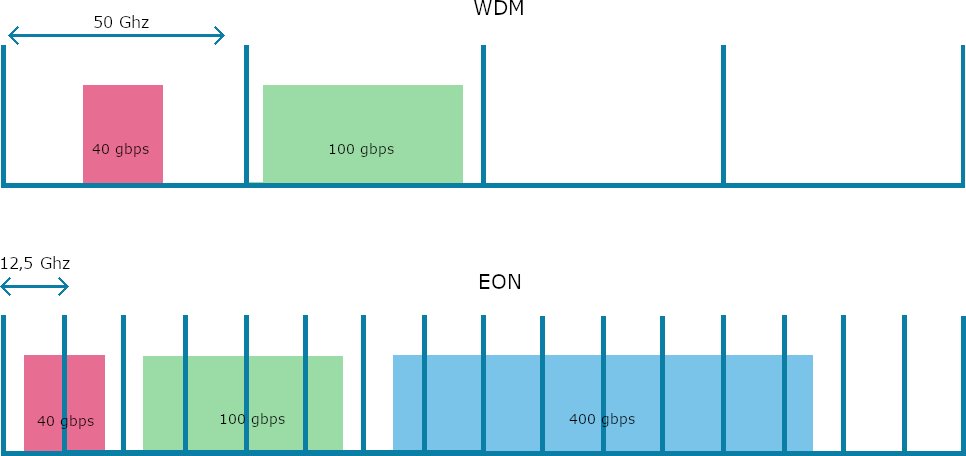
\includegraphics[width=0.95\textwidth]{capitulos/img/eonwdm.png}
% %     \caption{Redes WDM v s Redes EON}
% %     \label{fig:eonwdm}
% % \end{figure}


\section{Fragmentación del Ancho de Banda en MC-EON}
Las redes ópticas elásticas multinúcleo (MC-EON) permiten optimizar el uso del ancho de banda necesario para satisfacer una demanda, respetando tres restricciones fundamentales:
%

\begin{itemize}
    \item \textbf{Restricción de continuidad:} esta restricción implica que un cambio de luz o lightpath debe utilizar los mismos \textit{Frecuency Slots} (FS) a lo largo del camino establecido entre los nodos de origen y destino, tanto en la dimensión espectral como en la dimensión espacial (núcleo).
    \item \textbf{Restricción de consecutividad:} esta restricción establece que todos los FS utilizados para establecer un lightpath deben ser contiguos en el dominio espectral, formando un solo bloque contiguo de FS dentro del mismo núcleo. 
\end{itemize}
%

Estas restricciones conducen a que, tras sucesivas asignaciones y liberaciones de recursos, se genere la aparición de bloques aislados de FS no utilizados tanto en la dimensión espectral como en la dimesión espacial (núcleos) de los enlaces ópticos.
Dichos bloques fragmentados presentan desalineación tanto entre enlaces consecutivos de la ruta como entre los diferentes núcleos de una misma fibra multinúcleo. Como consecuencia, se incrementa significativamente la probabilidad de bloqueo de solicitudes, 
pudiendo la red rechazar demandas incluso cuando existe ancho de banda disponible suficiente en los enlaces. Este fenómeno se denomina \textbf{Fragmentación de la red} y en arquitecturas multinúcleo se manifiesta en dos domensiones complementarias:
%

\begin{itemize}
    \item \textbf{Fragmentación espectral:} se refiere a la presencia de bloques aislados de FS no utilizados en el dominio espectral, que no pueden ser aprovechados para establecer nuevas conexiones debido a las restricciones de continuidad y consecutividad.
    \item \textbf{Fragmentación espacial:} se refiere a la desalineación de bloques de FS disponibles entre los diferentes núcleos de una misma fibra multinúcleo, lo que dificulta la asignación eficiente de recursos en la dimensión espacial.
\end{itemize}
%

\textbf{Ejemplo ilustrativo del fenómeno:}
\begin{enumerate}[1 -]
   \item Se presenta el estado inicial del enlace mostrando las asignaciones activas de lightpaths distribuidos en los múltiples núcleos de la fibra.
   \item Se produce la liberación de recursos al finalizar el tiempo de vida de determinadas conexiones, generando segmentos espectrales disponibles dispersos en diferentes núcleos y posiciones del espectro.
   \item Se evidencia el rechazo de una nueva solicitud de conexión debido a que, pese a existir una cantidad agregada suficiente de FS libres en la red, estos no satisfacen simultáneamente las restricciones de contigüidad espectral dentro de un único núcleo y continuidad espacial a lo largo de la ruta. La conexión resulta bloqueada en todos los núcleos disponibles como resultado de la fragmentación tanto espectral como espacial inherente al sistema multinúcleo.  
\end{enumerate}
%

Para ilustrar estas restricciones, se presenta un ejemplo en las Figuras [] y [], donde se simula la conexión de una demanda de fod FS, con un nodo origen en 0 y un nodo destino en 3. En este escenario, existen dos posibblews caminos: 0-1-3 y 0-1-2-3.
%

La trayectoria de menor longitud corresponde a la ruta 0-1-3. No obstante, al procurar el establecimiento del lightpath mediante esta alternativa, la solicitud de conexión resulta denegada, dado que los enlaces 0-1 y 1-3 carecen de dos FS consecutivos y alineados espectralmente, tal como se evidencia en la Figura [].
%


\begin{figure}[H]
    \centering
    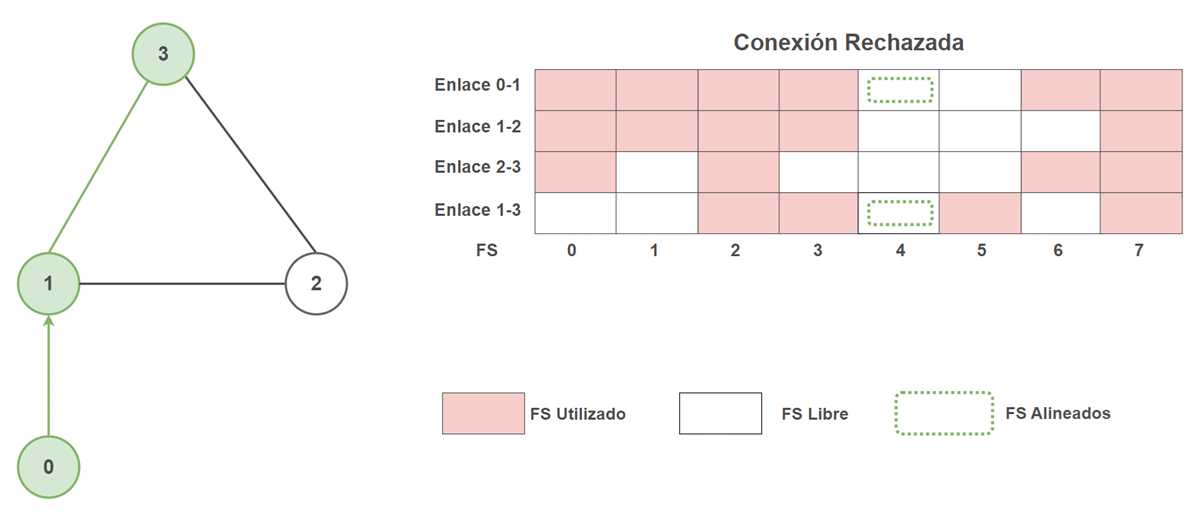
\includegraphics[width=1\textwidth]{capitulos/img/fragmentacionNuevo.png}
    \caption{Restricciones de contigüidad y continuidad aplicadas- Conexión Rechazada}
    \label{fig:fragmentacionNueva}
\end{figure}

\begin{figure}[H]
    \centering
    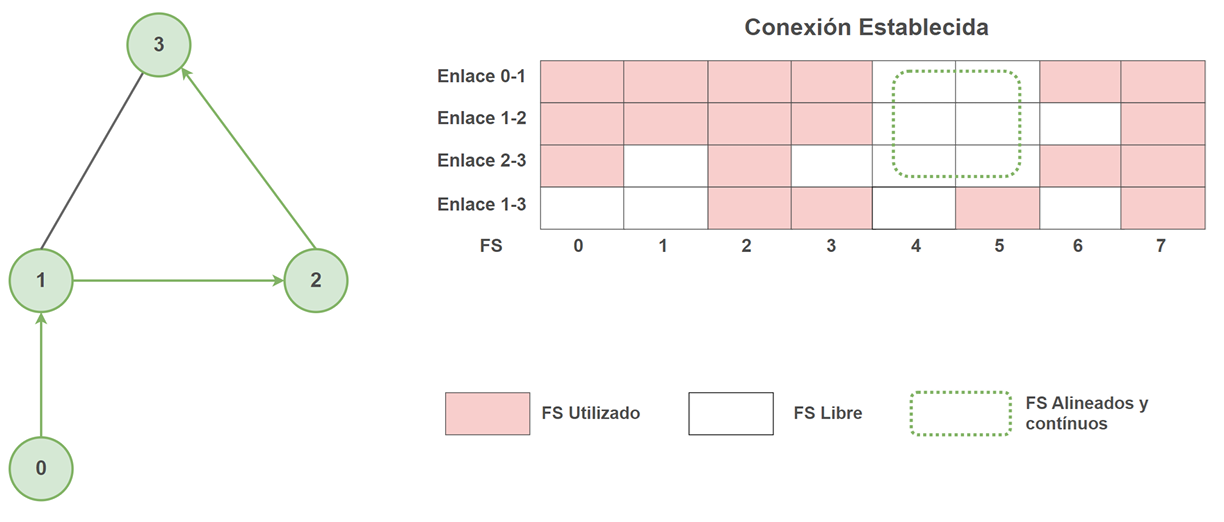
\includegraphics[width=1\textwidth]{capitulos/img/fragmentacion2Nuevo.png}
    \caption{Restricciones de contigüidad y continuidad aplicadas- Conexión Establecida}
    \label{fig:fragmentacion2Nueva}
\end{figure}

En contraste, al considerar la asignación del lightpath a través de la trayectoria de mayor extensión, específicamente 0-1-2-3, empleando los FS 4 y 5, la conexión se establece satisfactoriamente, puesto que esta configuración dispone de dos FS contiguos y alineados espectralmente, según se observa en la Figura [].
%

\subsection{Enfoques de gestión de fragmentación}
La problemática descrita previamente genera consecuencias perjudiciales para la infraestructura de red, ocasionando un incremento en la probabilidad de bloqueo y comprometiendo significativamente su desempeño óptimo y continuidad operacional. En consecuencia, resulta fundamental identificar estrategias que permitan prevenir, mitigar o reducir la fragmentación del espectro disponible.
%

De acuerdo con la bibliografía especializada, existen diversas aproximaciones que pueden ser consideradas para abordar la gestión de la desfragmentación. En la figura [] se presentan las principales estrategias de gestión de la fragmentación \cite{chatterjee2017fragmentation}.
%


La Desfragmentación constituye un procedimiento mediante el cual se ejecuta la reconfiguración o el re-ruteo de un subconjunto de conexiones existentes en la infraestructura de red. Su propósito fundamental consiste en reacomodar las asignaciones espectrales de las solicitudes de tráfico vigentes, consolidando de este modo los recursos disponibles en segmentos contiguos y continuos de mayor magnitud, los cuales pueden ser aprovechados para el establecimiento de futuras demandas \cite{talebi2014spectrum}.
%

Es factible abordar la problemática de la fragmentación prescindiendo de técnicas de desfragmentación espectral (Sin Desfragmentación), lo cual se alcanza mediante una administración del espectro orientada a la prevención de su fragmentación.
%

En el tratamiento de la fragmentación bajo un esquema Sin Desfragmentación, se pueden mencionar los algoritmos denominados Sensibles a la Fragmentación o \textit{Fragmentation Aware RSA} (FA-RSA). Estos consideran la fragmentación espectral durante el establecimiento de las demandas, empleando diversos indicadores de fragmentación, procurando así minimizar la fragmentación del espectro.
%

Alternativamente, es posible emplear técnicas de desfragmentación, las cuales se fundamentan en dos aproximaciones principales:
\begin{itemize}
         \item Desfragmentación Reactiva: El procedimiento se ejecuta como respuesta al bloqueo de una solicitud, con la finalidad de lograr su establecimiento exitoso.
         \item Desfragmentación Proactiva: Se lleva a cabo de manera periódica o en función de determinados umbrales que activan el proceso, permitiendo así reducir la fragmentación de la infraestructura de red y minimizar la ocurrencia de futuros bloqueos de solicitudes.
\end{itemize}
Las aproximaciones que implementan técnicas de desfragmentación pueden clasificarse además en: (i) estrategias sin re-ruteo, las cuales realizan únicamente una reasignación espectral en los \textit{lightpaths} o caminos ópticos establecidos, y (ii) estrategias con re-ruteo, que constituyen técnicas capaces de modificar tanto las rutas como el espectro asignado a los lightpaths existentes.
%

En el presente trabajo, para la gestión de la fragmentación se adoptó la aproximación con desfragmentación, de naturaleza proactiva y con re-ruteo de lightpaths preexistentes. En la figura [] se puede observar resaltada dicha estrategia.
%

\begin{figure}[H]
    \centering
    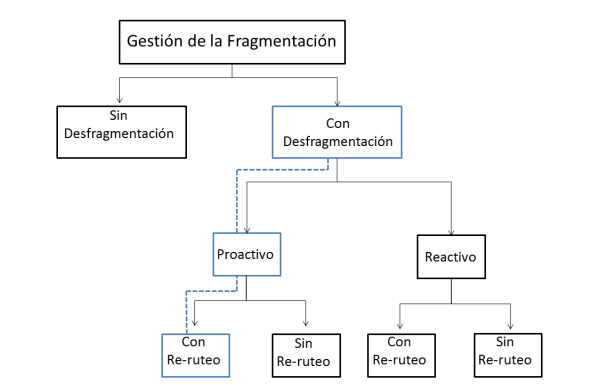
\includegraphics[width=1\textwidth]{capitulos/img/Gestion_Fragmentacion.PNG}
    \caption{Esquema de Gestión de la Fragmentación}
    \label{fig:gestion_fragmentacion}
\end{figure}
%


\section{Descripción del problema tratado}
La Fragmentación del Espectro en Redes Ópticas Elásticas Multinúcleo (Multi-Core EON) constituye una problemática que compromete la eficiencia en la utilización de recursos espectrales y espaciales. El desempeño de la infraestructura de red resulta severamente afectado, dado que este fenómeno puede ocasionar bloqueos de solicitudes debido a la ausencia de ranuras espectrales contiguas y alineadas entre enlaces consecutivos, así como por la indisponibilidad de núcleos adecuados, sin que necesariamente el espectro en todos los núcleos se encuentre completamente ocupado. En secciones previas se expusieron estrategias para el manejo de la fragmentación en la red; en el presente trabajo se examina la estrategia con desfragmentación, adoptando un enfoque proactivo.
%

Un método ampliamente implementado consiste en ejecutar el procedimiento de desfragmentación de manera periódica con el propósito de prevenir bloqueos futuros, abordando así una de las cuatro interrogantes planteadas por Zhang [], ¿Cuándo reconfigurar?.
%

En la figura [] se puede observar una posible solución a la problemática de la selección del momento óptimo para realizar la desfragmentación, la cual consiste en ejecutar desfragmentaciones periódicas en intervalos temporales fijos. En este caso, cada 100 unidades de tiempo, el eje vertical representa el volumen de tráfico cuantificado mediante el número de conexiones activas, mientras que el eje horizontal indica las unidades temporales; cada punto azul denota el instante en que el proceso de desfragmentación se ejecuta. Siguiendo este patrón, se evidencian situaciones donde se realizan procesos de desfragmentación cuando la red podría no requerirlos, considerando que la utilización de los recursos espectrales y de los núcleos constituye un indicador significativo del grado de fragmentación.
%

Además de la utilización de la red, existen otras métricas de fragmentación relevantes en redes multinúcleo, cuyos valores deben considerarse para el disparo de los procesos de desfragmentación, incluyendo la fragmentación por núcleo y la disponibilidad de recursos en la dimensión espacial.
%

De este modo, se evidencia la necesidad de un disparador inteligente para ejecutar el proceso de desfragmentación que considere todos estos parámetros o ``características'' para seleccionar apropiadamente el momento del disparo, dado que realizar múltiples desfragmentaciones de manera frecuente afecta directamente al desempeño de la red, pudiendo ocasionar disrupciones en las conexiones activas; mientras que ejecutar pocas desfragmentaciones muy dispersas resultaría en efectos prácticamente imperceptibles.
%

En síntesis, la selección del momento para ejecutar el proceso de desfragmentación resulta crítica debido a su impacto significativo en la cantidad de procesos de desfragmentación, lo cual incide directamente en las dos métricas globales más relevantes en el enrutamiento de redes ópticas elásticas multinúcleo: Cantidad de bloqueos y Cantidad de reconfiguraciones.
%

En los capítulos subsiguientes se presenta y aborda en profundidad un modelo de disparo inteligente que contempla numerosos factores tales como métricas de fragmentación de la red, utilización de recursos espectrales y espaciales, y bloqueos de solicitudes.
%

\begin{figure}[h!]
    \centering
    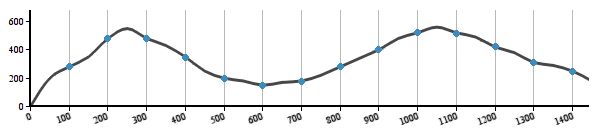
\includegraphics[width=1\textwidth]{capitulos/img/ejemploPeriodico.png}
    \caption{Ejemplo de desfragmentaciones periódicas con volumen de carga de tráfico variado}
    \label{fig:ejemploPeriodico}
\end{figure}
%


\section{Redes EON Multinúcleo}
Las redes EON Multinúcleo constituyen una variante avanzada de las redes EON que integran el concepto de fibras multinúcleo (MCF) para incrementar significativamente la capacidad de transmisión y la eficiencia espectral. Fundamentalmente, las redes EON Multinúcleo aprovechan múltiples núcleos independientes dentro de una misma fibra óptica para transmitir señales de forma simultánea y paralela, posibilitando una multiplicación de la capacidad de transmisión en comparación con las fibras convencionales [15].
 Estas características mencionadas en las EON Multinúcleo se materializan mediante la implementación de la Multiplexación por División de Espacio (SDM). Por esta razón, las redes EON Multinúcleo también se denominan SDM-EON[5]. En las redes EON Multinúcleo, se integra el concepto de asignación flexible de espectro con la utilización de múltiples núcleos, alcanzando una distribución más eficiente de la capacidad total de transmisión. Esta integración de tecnologías posibilita un incremento sustancial en la capacidad de transmisión a través de una única fibra, resultando esencial en un contexto donde la demanda de datos continúa creciendo de manera exponencial.
  Al incorporar el concepto de fibras multinúcleo en el diseño de las redes EON, se puede lograr una mayor adaptabilidad a las cambiantes necesidades del tráfico y una optimización más profunda de los recursos disponibles.
%

\begin{figure}[H]
    \centering
    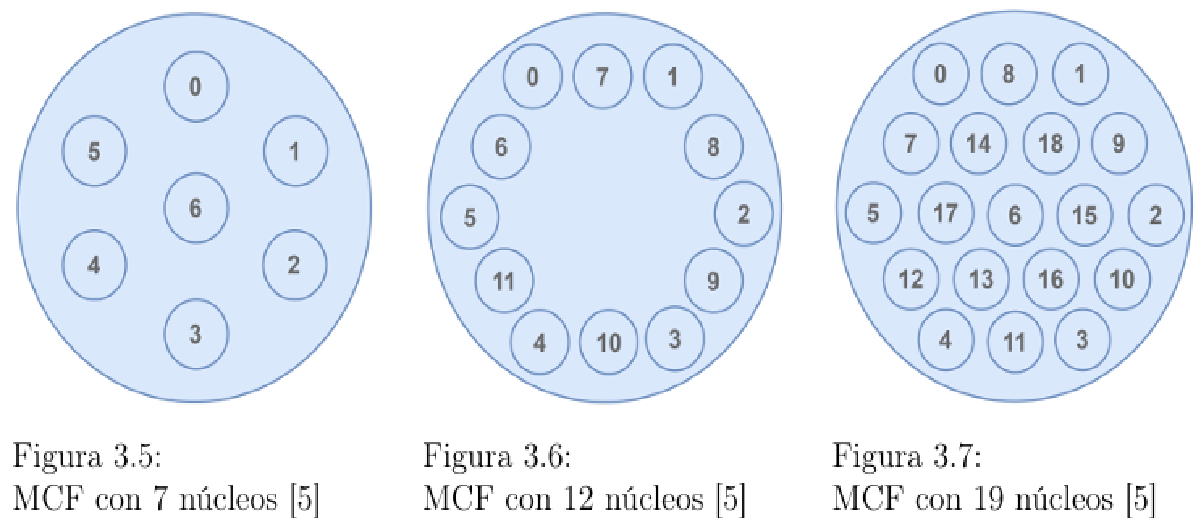
\includegraphics[width=1\textwidth]{capitulos/img/MCF_NUCLEOS.png}
    \caption{Ejemplo de Fibras Multinúcleo (MCF) con 7, 12 y 19 núcleos}
    \label{fig:MCF_NUCLEOS}
\end{figure}
%

Conforme a lo documentado en la literatura [], inicialmente podría considerarse que la utilización de redes EON con mayor cantidad de núcleos proporciona ventajas sustanciales debido a la amplia disponibilidad de recursos espectrales y espaciales. No obstante, se ha identificado que en las redes MCF, el principal desafío radica en la interferencia denominada diafonía (crosstalk), la cual se genera cuando una fracción de la potencia óptica de un núcleo se propaga hacia los núcleos contiguos.
 Este fenómeno ocasiona una interferencia significativa en los circuitos activos y complejiza considerablemente la asignación de las ranuras espectrales (FS). Investigaciones previas [] [] han indicado que para viabilizar la implementación de redes EON multinúcleo, resulta fundamental desarrollar fibras que minimicen la diafonía entre núcleos adyacentes.
%

 En la Figura [], se presenta una configuración de MCF con 7 núcleos dispuestos en un patrón hexagonal. En esta arquitectura, el núcleo central (núcleo N° 6) se encuentra rodeado por 6 núcleos adyacentes, resultando en una mayor incidencia de diafonía sobre este núcleo.
 En contraste, los núcleos periféricos (núcleos N° 0, 1, 2, 3, 4 y 5) poseen 3 núcleos adyacentes cada uno. La Figura [] exhibe una MCF con 12 núcleos organizados en una disposición anular. En esta configuración, cada núcleo presenta exactamente 2 núcleos adyacentes, lo que deriva en que todos los núcleos experimenten un nivel equivalente de diafonía.
 %

 Finalmente, la Figura [] ilustra una MCF con 19 núcleos. En este tipo de fibras, los núcleos pueden presentar hasta 6 núcleos adyacentes por núcleo, generando una mayor incidencia de diafonía.
%

\begin{figure}[H]
    \centering
    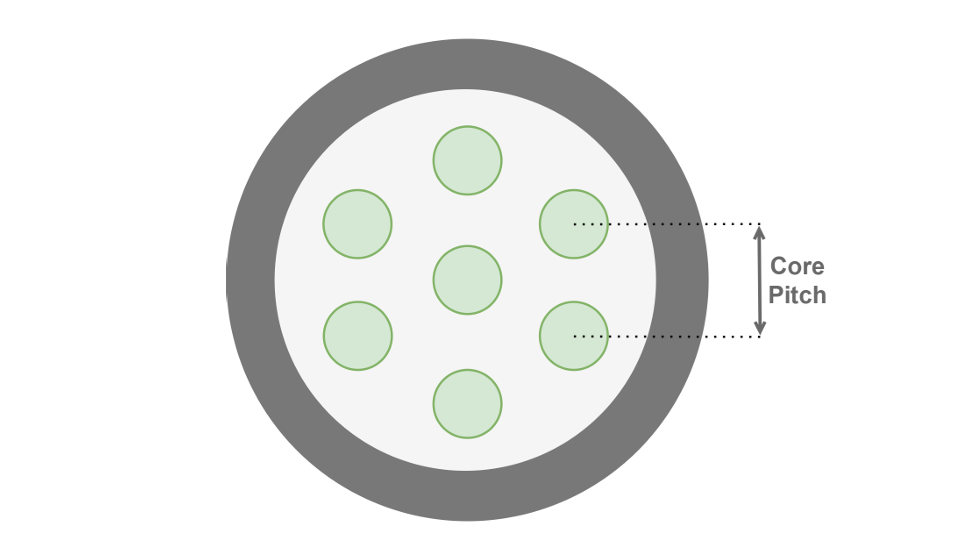
\includegraphics[width=1\textwidth]{capitulos/img/CORE_PITCH.png}
    \caption{Core Pitch entre dos núcleos adyacentes en un MCF de 7 núcleos}
    \label{fig:CORE_PITCH}
\end{figure}

\section{Diafonía en Redes Ópticas Elásticas Multinúcleo}
La diafonía constituye un fenómeno indeseado que se manifiesta en las redes de fibra óptica cuando la señal transmitida en una fibra se acopla hacia otra fibra contigua. En el contexto de las redes EON fundamentadas en MCF, la diafonía se define como la interferencia entre conexiones ópticas establecidas en núcleos adyacentes que emplean las mismas ranuras espectrales (FS) en un enlace común.
 Este tipo de interferencia se denomina diafonía entre núcleos o Inter-Core Crosstalk (XT). La interferencia ocasionada por el XT puede degradar la calidad de la señal en las FS afectadas, lo que implica que la señal en estas ranuras puede experimentar distorsiones, incrementando la probabilidad de errores en la transmisión de datos.
%
 
 Consecuentemente, impacta directamente en la capacidad de la red al «inhabilitar» estas FS para la transferencia de datos debido a la diafonía, generando espacios no utilizables entre ellas.
%

 En síntesis, esto deriva en una reducción de la cantidad total de FS disponibles para la transmisión de datos, limitando la capacidad operativa de la red. Con menor disponibilidad de FS, se reducen los canales para transmitir datos, lo que puede restringir la capacidad total de transmisión de la infraestructura de red.
%

 En las redes SDM-EON, el XT entre dos núcleos de una MCF depende significativamente de la distancia entre dicho par de núcleos, denominada core pitch ($\Lambda_{i,j}$). A mayor core pitch, menor será el impacto del XT entre estos dos núcleos [].
 No obstante, resulta importante destacar que, a medida que se incrementa el core pitch, la capacidad de la fibra óptica disminuye. Es decir, al aumentar la distancia física entre dos núcleos, se reduce el espacio disponible en la fibra óptica para albergar núcleos adicionales.
 Por consiguiente, resulta fundamental establecer un equilibrio entre un core pitch reducido para incrementar la capacidad y uno suficientemente amplio para minimizar los efectos del XT. Este balance posibilita optimizar el desempeño y la eficiencia de la red.
 %

\begin{figure}[H]
    \centering
    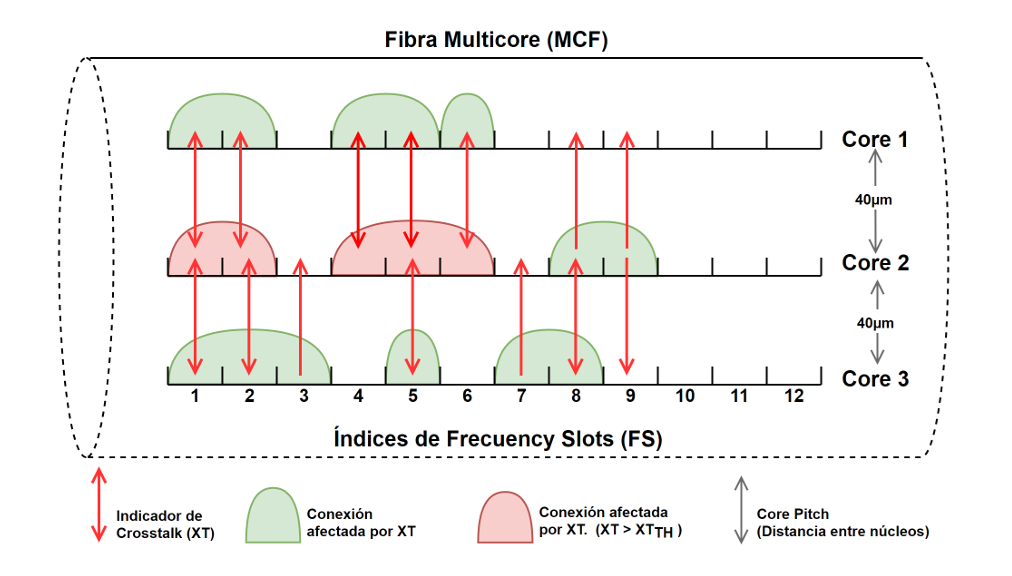
\includegraphics[width=1\textwidth]{capitulos/img/XT_MCF.png}
    \caption{XT en un Fibra MCF de 3 núcleos []}
    \label{fig:XT_MCF}
\end{figure}
%

Para demostrar el comportamiento del crosstalk (XT) entre núcleos en fibras multinúcleo, se analiza el ejemplo presentado en la figura [], la cual ilustra una fibra óptica multinúcleo (MCF) compuesta por tres núcleos organizados en configuración lineal.
En esta topología, resulta evidente que el núcleo central (núcleo 2) experimenta una interferencia significativa por XT intercore. Este fenómeno se atribuye a que ambos núcleos contiguos (núcleos 1 y 3) mantienen conexiones establecidas en intervalos espectrales similares a aquellos ya ocupados en el núcleo 2.
A modo de ejemplo, los segmentos espectrales FS1 y FS2 resultan inutilizables en el núcleo 2 debido a la interferencia generada por las asignaciones activas en los núcleos laterales.
Esta misma situación se replica en los intervalos FS4, FS5 y FS6 del núcleo mencionado. Consecuentemente, en arquitecturas SDM-EON basadas en fibras multinúcleo, resulta imperativo evaluar el impacto del XT intercore durante el proceso de asignación de recursos espectrales, a fin de mitigar degradaciones en la calidad de transmisión.

Es relevante destacar que el crosstalk intercore no afecta exclusivamente a los segmentos espectrales con demandas activas, sino también a aquellos recursos disponibles en núcleos adyacentes. Un análisis detallado de la figura [] revela que incluso los intervalos espectrales sin conexiones asignadas experimentan interferencia procedente de transmisiones en núcleos contiguos.
 Esto se ejemplifica con los segmentos FS8 y FS9 del núcleo 1, que sufren degradación por el XT generado desde las mismas posiciones espectrales en el núcleo 2. En determinadas circunstancias, esta interferencia puede superar el umbral de crosstalk admisible, imposibilitando la utilización de dichos recursos para el establecimiento de futuras conexiones en arquitecturas multinúcleo.

 %\section{Análisis Bibliográfico}     
% El trabajo presentado por M. Quagliotti \cite{quagliotti2017spectrum} propone un algoritmo RSA que busca mantener bajo el índice de fragmentación mediante el uso de una heurística básica durante la asignación del espectro, también brinda una amplia y útil descripción de métricas para evaluar la fragmentación del espectro.

% Para recopilar el conjunto de métricas de fragmentación utilizadas, realizaron un extenso estudio de la literatura científica, las cuales son: Utilization Entropy (UE), Shannon Entropy (SHF), External Fragmentation (EF), Access Blocking Probability (ABP), Compactness (SC) y High-slot Mark (HSM).

% Cada métrica de fragmentación proporciona su propia y peculiar medida de ocupación del espectro, relacionadas a la accesibilidad de recursos para el caso de EF, y ABP, grado de desorden y entropía en UE y SHF y compacidad del espectro ocupado en SC.

% Para nuestra investigación utilizamos algunas de las métricas presentadas en el mencionado articulo, las cuales nos sirven como características esenciales en la construcción de nuestro modelo de predicción de probabilidades de bloqueo.  

% Seguidamente presentamos un análisis bibliográfico de trabajos presentes en el estado del arte que abordaron el mismo problema.

% Jaume Comellas, Laura Vicario, y Gabriel Junyent \cite{comellas2018periodic} nos presentan un análisis de la desfragmentación periódica en redes EON con un tráfico dinámico, evaluando los diferentes efectos de los parámetros de desfragmentación en el rendimiento de la red.

% El enfoque presentado en el trabajo consiste en realizar las desfragmentaciones en periodos fijos de N unidades de tiempo, con el principal objetivo de encontrar valores adecuados de N, ya que periodos de desfragmetación muy pequeños implican tener el espectro tan compactado como sea posible, pero a expensas de ejecutar el algoritmo con demasiada frecuencia, lo cual añade complejidad al proceso. Por otro lado, para valores muy altos de N, los efectos de la desfragmentación son insignificantes.

% Este tipo de desfragmentaciones en periodos fijos es utilizado ampliamente en distintas investigaciones tales cómo \cite{davalos2019spectrum}, \cite{luo2012partial}, entre otros. En nuestra investigación utilizamos esta técnica a fin de comparar los resultados con el disparador que proponemos.

% Otra manera de afrontar el enfoque proactivo del proceso de desfragmentación es realizarlo mediante algún tipo de disparador de tal manera que la misma sea ejecutada solo en periodos de tiempo donde es realmente necesaria, a continuación, veremos algunos artículos los cuales usaron esta estrategia.

% La investigación realizada por Yutaka Takita y colegas \cite{takita2016wavelength} propone un mecanismo de disparo para el proceso de desfragmentación basado en el valor del \textit{High-slot Mark} (HM) el cual indica el número máximo de una ranura ocupada en la red. Utilizan esta métrica ya que lo consideran como una medida válida para evaluar la eficiencia en la utilización de los recursos. El proceso de desfragmentación se dispara de manera aleatoria cuando el valor del HM es mayor a un valor de \( HM_{max} \) definido previamente, en el artículo mencionado utilizan 30 como valor para \( HM_{max} \). 

% Para el proceso de disparo en nuestro método propuesto se utilizan un conjunto de características o parámetros que indican el estado actual de la red, parte de ellas al igual que el \textit{High-slot Mark} son también métricas que indican la fragmentación del espectro. En el capitulo 4 se explican en profundidad estas características donde una de ellas es el llamado \textit{Maximum Slot Index} (MSI) el cual tiene una definición equivalente al del \textit{High-slot Mark}. 

% Otra propuesta para el disparo es presentada por Ricardo V. Fávero y colegas \cite{favero2015new}. En su método combinan el enfoque reactivo y el enfoque proactivo para determinar el periodo en el que será ejecutado el proceso de desfragmentación, en la figura \ref{fig:favero} se puede observar el diagrama que ilustra el algoritmo propuesto.

% Inicialmente la variable \textit{d} que utilizan para representar el estado de fragmentación se coloca en 0, el proceso de desfragmentación (DS) se ejecuta al cumplirse alguna de las siguientes condiciones.

% Si se intenta establecer una demanda y no se encuentra un camino disponible para la misma, se verifica la variable \textit{d}, si esta se encuentra en 0 se ejecuta el proceso \textit{DS}, si no se logra establecer la demanda aun después del proceso de desfragmentación la misma se bloquea y la variable \textit{d} se cambia a 1.

% La otra posibilidad de ejecución es cuando se intenta liberar una demanda, se ejecuta el proceso \textit{DS} sí \textit{d} = 1 y si la cantidad de \textit{lighpaths} liberados (\textit{r}) es igual a la variable predefinida previamente \textit{R}. 

% Como se puede ver el método propuesto considera principalmente las conexiones liberadas por lo que puede considerarse como periódica.


% \begin{figure}[h!]
%     \centering
%     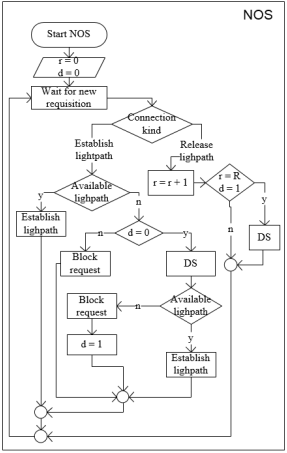
\includegraphics{capitulos/img/disparoFavero}
%     \caption{Algoritmo propuesto por Favero y colegas \cite{favero2015new}}
%     \label{fig:favero}
% \end{figure}

%Mingyang Zanhg y colegas plantean en su investigación \cite{zhang2013bandwidth} un disparo para el proceso de desfragmentación basado en la cantidad de conexiones liberadas. Básicamente consiste en ejecutar la desfragmentación cuándo la cantidad de conexiones liberadas es igual al parámetro fijo \textit{TH} (\textit{Threshold}). En su investigación utilizaron 300 como valor de \textit{TH}.

%El trabajo presentado por Jie Zhang y colegas \cite{zhang2012priority}, proponen un disparo basado en el concepto de \textit{Spectrum Compacteness} o Compacidad del Espectro (SC) el cual es una métrica de fragmentación.

%Para determinar el momento del disparo para el proceso de desfragmentación tienen en cuenta los siguientes pasos:  
% \begin{enumerate}[label=\arabic*)]
%     \item Seleccionar un valor apropiado de \textit{Spectrum Compactness} (SC) para actuar como umbral (T) para el disparo de la desfragmentación.
%     \item Actualizar el valor de SC después de liberar conexiones o al establecer una nueva conexión. 
%     \item Comparar los valores de SC y T; si SC < T disparar la desfragmentación y pasar al siguiente paso, sino volver al paso 2.
%     \item Actualizar el ultimo valor de SC después de la desfragmentación y volver al paso 3.
% \end{enumerate}

% Por último el trabajo propuesto por Zhang y colegas \cite{zhang2014dynamic} presentan un análisis del problema de la desfragmentación de redes EON dividido en cuatro sub-problemas, el tercero de ellos es ¿Cuándo reconfigurar?.

% Para el tercer subproblema plantean un algoritmo de disparo el cual tiene en cuenta la probabilidad de bloqueo instantánea (B) en un periodo \(\Delta \)t \((B(\Delta t))\) y la utilización del ancho de banda. 
% De esta forma buscan realizan la comparación entre \(B(\Delta t)\) con \(B_{th}\) (umbral de probabilidad de bloqueo para el disparo del proceso de desfragmentación) solo cuando la red se encuentra con un crecimiento en la utilización del ancho de banda. 
\newpage


\chapter{ Aprendizaje Automático }
Aprendizaje Automático o \textit{Machine Learning} es una rama de la inteligencia artificial, el cual construye un modelo matemático basado en datos de muestra, conocidos como datos de entrenamiento, de forma a realizar predicciones o tomar decisiones sin que haya sido programado de forma explícita para realizar dicha tarea.\cite{zhang2020matrix}

Una definición más orientada a la ingeniería podría ser:

Se dice que un programa de computadoras aprende de una experiencia E respecto a una tarea T y alguna forma de medida de rendimiento P, si el rendimiento en la tarea T, medido por P, mejora con la experiencia E.\cite{mitchell1997machine}

Para entender un poco mejor utilicemos un ejemplo de un programa de aprendizaje automático, como podría ser un filtro de spam de correos electrónicos. Este filtro de spam puede aprender a detectar y marcar los correos mediante ejemplos proveídos por los usuarios, tanto de aquellos correos que el usuario marcó como un spam, así como de correos que el usuario considera que no lo son. Estos datos de ejemplo que el programa puede utilizar para aprender de ellos son llamados conjuntos de entrenamiento.

Para este caso la tarea T es la de marcar nuevos correos electrónicos como spam, la experiencia E es el entrenamiento con los datos, y la medida del rendimiento P podría ser la proporción de acierto o \textit{Accuracy} de los correos correctamente clasificados como spam o no.

\section{Tipos de sistemas de aprendizaje automático}
Los sistemas de aprendizaje automático pueden clasificarse de acuerdo a la cantidad y el tipo de supervisión que necesitan durante la fase de entrenamiento. Existen 3 grandes categorías de las cuales hablaremos a continuación:

\begin{itemize}
    \item Aprendizaje supervisado: En este tipo de aprendizaje, el conjunto de entrenamiento que se provee al programa incluye las soluciones deseadas, a estas soluciones se les conoce como etiquetas o \textit{labels}. Este método aprende una regla general la cual mapea el conjunto de entradas con las salidas deseadas.
    En el aprendizaje supervisado podemos dividir las tareas en dos enfoques principales, la Clasificación y Predicción de un valor numérico generalmente realizado por medio de la Regresión. 

    \begin{itemize}
        \item Clasificación: Consiste en brindar ejemplos de entradas indicando a que clase o clases pertenece, de forma a poder realizar el entrenamiento y de esa forma para nuevas entradas poder clasificar dentro de alguna de las clases contempladas.
        \item Predicción: Consiste en brindar datos de entrada con un conjunto de características y un valor objetivo, de forma que con el entrenamiento para las nuevas entradas es posible predecir el valor objetivo a partir del conjunto de características. Este tipo de tareas se lo conoce como Regresión.
    \end{itemize}
    \item Aprendizaje No-supervisado: En este tipo de  aprendizaje, el conjunto de entrenamiento que se provee al programa no incluye las soluciones deseadas o conocidas. La principal tarea de este método es la de encontrar soluciones por si mismo (por ejemplo, patrones o estructuras en los datos).
    \item Aprendizaje por refuerzo: Al tipo de aprendizaje basado en la retroalimentación se lo conoce como aprendizaje por refuerzo. En este método los datos de entrenamiento son proveídos en forma de recompensas (positivas o negativas) por medio de la retroalimentación a un agente de inteligencia artificial que interactúa con un entorno dinámico. La retroalimentación entre sistema de aprendizaje y la experiencia obtenida por el agente es muy útil para mejorar el rendimiento en la tarea que está aprendiendo.
\end{itemize}

\section{Redes Neuronales Artificiales}
Las redes neuronales artificiales son algoritmos bio-inspirados, es decir, están vagamente inspirados en el cerebro biológico. Como ocurre en el cerebro, las redes neuronales artificiales consisten en unidades simples llamadas neuronas las cuales se encuentran interconectadas entre si. Estas reciben, procesan y transmiten señales a otras neuronas actuando como un interruptor.

Los elementos de una red neuronal son bastantes simples, la complejidad y el poder de estos sistemas proviene de la interacción entre sus elementos. Por ejemplo, el cerebro humano cuenta  con más de cien mil millones de neuronas y cien billones de conexiones.

\subsection{Perceptrón}
El concepto de perceptrón se encuentra inspirado en las neuronas biológicas, cuya tarea principal es la de bloquear o dejar pasar las señales. Las neuronas reciben estas señales eléctricas, si la señal sobrepasa cierto umbral, la neurona lanza una señal de salida. \\
\begin{figure}[H]
    \centering
    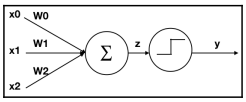
\includegraphics{capitulos/img/perceptron.png}
    \caption{Comportamiento del perceptrón}
    \label{fig:perceptron}
\end{figure}
Un perceptrón busca imitar ese mismo comportamiento, de la manera en la que se muestra en la figura \ref{fig:perceptron}. El mismo puede recibir múltiples datos de entrada \(X = {x_{0},x_{1},x_{2},...,x_{n}}\), entonces estos datos son multiplicados por un conjunto de pesos \(W = {w_{0},w_{1},w_{2},...,w_{n}}\). La suma ponderada z de estos datos de entrada, pasa por una función de activación, devolviendo así un valor y dependiendo del tipo de función de activación. También es posible expresarlo matemáticamente por medio de la siguiente fórmula: 
\begin{equation}
z = \sum_{i=1}^{n} w_{i} x_{i} = w^{T}x
\end{equation}
Este es el modelo matemático de una neurona, representado como una suma explícita y como una operación matricial. El término \(w^{T}x\)  es la representación vectorizada de la fórmula, donde \textit{w} es el peso de la matriz que primeramente es transpuesta y luego es multiplicada por un vector de entradas \textit{x}. Para obtener una descripción matemática completa podríamos añadir una constante \textit{b}, llamado bias.
\begin{equation}
z = \sum_{i=1}^{n} w_{i} x_{i} + b = w^{T}x + b
\end{equation}
Con esto obtenemos una expresión genérica de una ecuación lineal, el cual es  todo el proceso previo a su paso por la función de activación, la cual determinara si el perceptrón deja pasar la señal.
Existen muchas variantes para la función de activación, La función de activación mas sencilla es la función de paso. La salida de la neurona será aproximada por esta función, la cual se expresa por medio de la siguiente ecuación:
\begin{equation}
f(x)=\left\lbrace\begin{array}{c} 1~~~si~ (w^{t} x+b) > 0 \\ 0~~~caso~contrario~~ \end{array}\right.
\end{equation}

\subsection{Funciones de activación}
Existen varios tipos de funciones de activación, donde dependiendo de la tarea o valor buscado, estas pueden ser más o menos útiles. A su vez, estas funciones usualmente son utilizadas para agregar la no-linealidad, ya que sin esto solo podríamos tener soluciones lineales. Algunas de las funciones de activación más utilizadas son la sigmoide, tanh y la relu (\textit{rectified linear unit}) los cuales se muestran en la figura \ref{fig:funcionesActivacion}
\begin{figure}[h!]
    \centering
    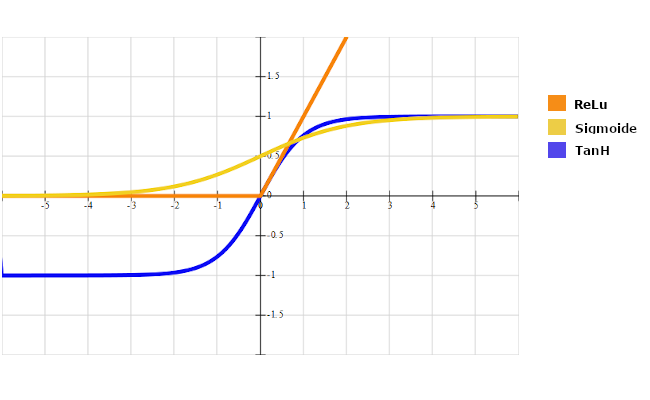
\includegraphics[width=1\textwidth]{capitulos/img/funcion_activacion.png}
    \caption{Funciones de Activación}
    \label{fig:funcionesActivacion}
\end{figure}
\newpage
\subsection{Arquitectura y aprendizaje}
Si muchas neuronas son conectadas entre sí, una red neuronal artificial es creada. En general, toda neurona de la red neuronal artificial está asociada a una capa. Cada neurona está conectada a todas las neuronas de la capa anterior y de la siguiente. Estas conexiones están ponderadas por un peso.\\
Un ejemplo de una arquitectura de redes neuronales artificiales se puede observar en la figura \ref{fig:redNeuronal}, donde se encuentra divida en tres áreas. La primera área contiene a la capa de entrada, y es la encargada de recibir y alimentar a la red con los datos de entrada. El área intermedia está conformada por una o más capas y son conocidas como capas ocultas, donde el número de capas ocultas determina la profundidad de la red. Por último, la última área contiene a la capa de salida que dependiendo de la tarea puede tener uno o más neuronas de acuerdo a los posibles valores de salida.\\
\begin{figure}[H]
    \centering
    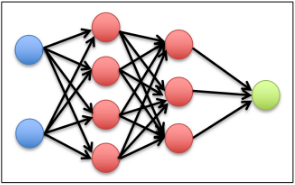
\includegraphics{capitulos/img/redNeuronal.png}
    \caption{Ejemplo de red neuronal}
    \label{fig:redNeuronal}
\end{figure}
Una vez que el peso de cada una de las conexiones de la red es establecido, es posible calcular un valor de salida para cada entrada de la red neuronal. En la mayoría de los casos, los pesos son establecidos de manera aleatoria por lo que los valores de salida calculados pueden ser diferentes a lo esperado. La idea es ajustar estos pesos de manera individual de forma a que el error cuadrático medio entre los valores calculados y los valores esperados sean mínimos, esto se realiza por medio del método de retropropagación o \textit{backpropagation}.\\

Primeramente, se calcula el resultado para un registro del conjunto de datos conocido, luego se calcula el error entre el resultado calculado y el resultado esperado. El error es propagado hacia atrás, pasando por todas las capas, empezando por la última capa y terminando con los pesos individuales de la primera capa de la red neuronal. La distribución del error toma lugar como una función de los valores de los pesos individuales. Una vez que los pesos individuales son cambiados, se procede a realizar el mismo procedimiento con un nuevo registro del conjunto de datos.\\

Para minimizar el error, se utiliza el método de descenso del gradiente, el cual al igual que el algoritmo de retropropagación son explicados en detalle en \cite{rashid2016make}.\\

Por otro lado tenemos el ratio de aprendizaje o \textit{Learning Rate} el cual es un indicador de cuánto cambian los pesos en cada iteración, Un valor de \textit{Learning rate} alto nos acerca de forma más rápida al error mínimo, pero una valor más bajo puede converger mejor. En la mayoría de los casos los valores elegidos son de 0.001 a 0.3.\\

Generalmente el entrenamiento de una red neuronal artificial con un solo conjunto de datos no es suficiente para alcanzar el mínimo error de salida, esto especialmente para valores bajos de \textit{Learning Rate}. Para mejorar esto, se realizan varias pasadas del conjunto de datos completo a través de la red neuronal, a cada pasada se lo conoce como época o \textit{epoch}. 

\section{Aplicación de Machine Learning en Redes Ópticas Elásticas}

En esta sección presentamos un estudio bibliográfico  del estado del arte de algunas técnicas de \textit{Machine Learning} aplicadas a problemas existentes en redes ópticas elásticas.

Panchali Datta Choudhury y Tanmay De, nos presentan un analisis del estado del arte  del uso de técnicas de \textit{Machine Learning} en redes ópticas elásticas \cite{choudhury2019recent}.

Algunas de las áreas presentadas por los autores en donde actualmente se utilizan estas técnicas son las siguientes:



\begin{itemize}
    \item Evaluación o predicción de la calidad de servicio
    
    Investigaciones como la propuesta en \cite{panayiotou2019data}, presenta un modelo de asignación de ancho de banda en EON teniendo en consideración los requisitos de la calidad del servicio o \textit{Quality of Service} (QoS) de la red. Utilizando la técnica de Aprendizaje Reforzado o \textit{Reinforcement Learning} para resolver el problema de asignación de ancho de banda, donde la función de recompensa para el modelo de aprendizaje reforzado se basa en el cumplimiento o no de los requisitos de QoS.
    
    \item Supervivencia
    
    Se hace uso del aprendizaje por refuerzo profundo en el trabajo \cite{luo2019leveraging}, explorando el problema de optimización de una red en general teniendo en cuenta la capacidad de supervivencia de la misma. Para ello se utilizó un enfoque de aprendizaje por refuerzo profundo, utilizando dos agentes, en donde uno de ellos se utiliza para proporcionar un esquema de trabajo y el otro se encarga de proporcionar el esquema de protección, de esta manera la combinación de ambos sumado a un enfoque de recompensas para aumentar la rentabilidad nos brinda una solución para las políticas de asignación de espectro, modulación y enrutamiento que además nos provea de  supervivencia.
    
    \item Predicción de tráfico
    
    El trabajo presentado por Aibin \cite{aibin2018traffic} para la predicción de tráfico en redes de centro de datos en la nube o \textit{Cloud Data Center Networks} utiliza un enfoque de árbol de búsqueda de Monte Carlo. Para una solicitud particular, esta técnica de búsqueda identifica el centro de datos en la nube más apropiado y la combinación de rutas candidatas para enrutar las solicitudes. Para lograr esto se crea un árbol disperso realizando la selección por medio del método de Monte Carlo.
    
    \item Enrutamiento, modulación y asignación del espectro
    
    En \cite{chen2018deep}, los autores proponen un modelo de aprendizaje reforzado profundo, con el objetivo de desarrollar un modelo autónomo de RMSA en redes ópticas elásticas, utilizando redes neuronales convolucionales también conocidas como \textit{Q Networks} para aprender las políticas RMSA considerando la conectividad, utilización del espectro y solicitudes de tráfico en redes EON.
    
    
\end{itemize}

En el área de interés de este trabajo, nos encontramos con algunos trabajos enfocados a la solución del problema de la fragmentación, pero enfocados en otro tipo de redes, como el presentado en \cite{trindade2020machine}, el cual se encuentra enfocado en \textit{Space Division Multiplexing Elastic Optical Networks} o SDM-EON , utilizando redes neuronales, específicamente una conocida como red neuronal de Elman, para la predicción de tráfico de forma a mitigar la fragmentación y el problema de \textit{Cross-talk}.

Para este tipo de redes también contamos con un algoritmo de desfragmentación basado en Machine Learning \cite{xiong2019machine}. Los autores proponen un algoritmo de desfragmentación utilizando un enfoque de aprendizaje no supervisado, por lo que no requiere de conocimientos previos de la red. El algoritmo se encarga de identificar aquellos \textit{lightpaths} que pueden ser agrupados en base a ciertas características, para luego mapear esos grupos a los núcleos y reordenar al espectro sin necesidad de realizar re-ruteos.




\chapter{ Método Propuesto }
Este trabajo propone una solución para la selección del momento de disparo de procesos proactivos de desfragmentación en redes EON, basado en técnicas de \textit{Machine Learning} para los cuáles predicen la probabilidad de bloqueo de una demanda \textit{unicast} en un momento determinado \textit{t}.

Para esta predicción se utiliza un modelo de regresión basado en redes neuronales, utilizando un conjunto de datos de simulaciones de tráfico \textit{unicast} en diversas topologías de redes EON, tomando parámetros o características relacionadas a la fragmentación y la utilización de la red como datos de entrada y produciendo un valor estimado de la probabilidad de bloqueo. Se fija además un valor límite de probabilidad para la realización del proceso de desfragmentación.

\section{Características}

En el área de \textit{Machine Learning}, se conoce cómo ``características'' a los parámetros o datos de entrada del modelo de aprendizaje.

Las características seleccionadas fueron aquellas que se encuentran relacionadas al uso y la fragmentación de la red, así como también al bloqueo de las demandas. Se tomaron las principales métricas usadas para la determinación del estado de fragmentación, de acuerdo con \cite{quagliotti2017spectrum}, además de otras relacionadas a la utilización de la red. 

Estas características son las siguientes: 

\begin{itemize}
    \item Entropía de utilización\cite{wang2012utilization}: La entropía de utilización es una métrica de fragmentación de enlaces de la red.  Un valor bajo de entropía indica que el ancho de banda de los enlaces de fibra óptica está siendo usado de forma ordenada, con menos bloques de FS utilizados o no utilizados, y con un nivel de fragmentación menor.
    La entropía de un enlace está definida como:
    \begin{equation}
        Ent_{link} = \sum_{i=1}^{N-1} FS_{i} \oplus FS_{i + 1}
    \end{equation}
    donde N es la cantidad de FS en el enlace, \(FS_{i}\) representa al FS de índice i dentro del enlace, y tiene valor 1 si el FS está ocupado, y valor 0 en caso contrario, y se realiza una operación XOR sobre FS contiguos del enlace.
    Para obtener la entropía de la red se calcula el promedio de la entropía en cada enlace:
    \begin{equation}
        Ent_{red} = \sum_{i=1}^{\left | E \right |} \frac{Ent_{link - i}}{{\left | E \right |}}
    \end{equation}
    \item Entropía de Shannon (SHF)\cite{wright2015minimum}: Es una métrica de fragmentación de enlaces, que es una variación de la anterior característica, definida por.
    \begin{equation}
        SHF_{link} = \sum_{i=1}^{B} \frac{S_{i}^{free}}{N}~ln\frac{N}{S_{i}^{free}}
    \end{equation}
    Donde \(S^{free}\) representa la cantidad de FS libres en el enlace y \textit{B} la cantiadad de bloques de FS libres. Para calcular el SHF de la red se calcula el promedio de los valores calculados en todos los enlaces.
    \begin{equation}
        SHF_{red} = \sum_{i=1}^{\left | E \right |} \frac{SHF_{link - i}}{{\left | E \right |}}
    \end{equation}
    \item \textit{Bandwidth Fragmentation Ratio} o Relación de Fragmentación de ancho de banda o  (BFR)\cite{zhang2013bandwidth}: Representa el índice de fragmentación de los recursos de la red. El BFR de un link se define como:
    \begin{equation}
        BFR_{link} = 1 - \frac{MaxBlock()}{S^{free}}
    \end{equation}
    Donde \textit{MaxBlock()} es el tamaño del mayor bloque de FS libres y \(S^{free}\) es la sumatoria total de FS libres en el enlace \textit{link}.
    El BFR de la red podemos calcular de la siguiente manera.
    \begin{equation}
       BFR_{red} = \sum_{i=1}^{\left | E \right |} \frac{BFR_{link - i}}{{\left | E \right |}}
    \end{equation}
    \item \textit{Maximum Slot Index} o Mayor Índice de FS utilizado (MSI): Este valor indica el valor del índice de FS más alto que está siendo utilizado dentro de un enlace.
    Para calcular el MSI de la red, se halla el índice máximo usado en todos los enlaces de la red y se calcula el promedio:
    \begin{equation}
        MSI_{red} = \sum_{i=1}^{\left | E \right |} \frac{MSI_{link - i}}{{\left | E \right |}}
    \end{equation}

    Donde  \(MSI_{link} - i\) es el mayor índice utilizado en el enlace i.
    \item Consecutividad del espectro (CE)\cite{wang2012spectrum}: Este valor refleja la alineación de los FS en un camino en particular, para obtener el valor para un camino en particular aplicamos la siguiente fórmula.
    \begin{equation}
        CE = \frac{Joins}{Bloques} \times \frac{S_{free}}{  N  }
    \end{equation}
    Donde \textit{Joins} se calcula como la cantidad total de bloques de dos FS libres adyacentes distintos dentro del enlace, \textit{Bloques} es la cantidad de bloques de FS libres en el enlace y \(S_{free}\) es la cantidad de FS libres en el enlace.
    Y para calcular la consecutividad en una red se calculan previamente todos los caminos de dos enlaces en la red, y luego se calcula el valor de la consecutividad para todas esas rutas y al final se halla el promedio.
    \begin{equation}
        CE{red} = \sum_{i=1}^{\left | K \right |} \frac{CE_{link - i}}{{\left | K \right |}}
    \end{equation}
    donde \(CE_{link - i}\) representa la consecutividad de la ruta de dos enlaces i calculada previamente, y K es la cantidad de rutas de dos enlaces que existen en la red. 
    \item Utilización de la Red: Se define como el cociente entre la sumatoria de todas las FS ocupados con la cantidad total de FS.
    \begin{equation}
        Uso_{link} =  \frac{sum(i)}{N}
    \end{equation}
    Donde \(sum(i)\) es la cantidad de FS utilizados en el enlace \(i\) y \(N\) es la cantidad total de FS en el enlace. 
    
    \begin{equation}
        Uso_{red} = \sum_{i=1}^{\left | E \right |} \frac{Uso_{link -i}}{\left | E \right |}
    \end{equation}
    
    \item Acumulación de FS bloqueados: Valor que muestra la sumatoria de las FS requeridos por demandas bloqueadas en las D demandas anteriores al periodo de tiempo actual.
    \begin{equation}
        FSB = \sum_{i=1}^{D} S_{i}^{block}
    \end{equation}
    Donde \(S_{i}^{block}\) es la cantidad de FS solicitados por la demanda bloqueada i.
\end{itemize}

\begin{figure}[!h]
    \centering
    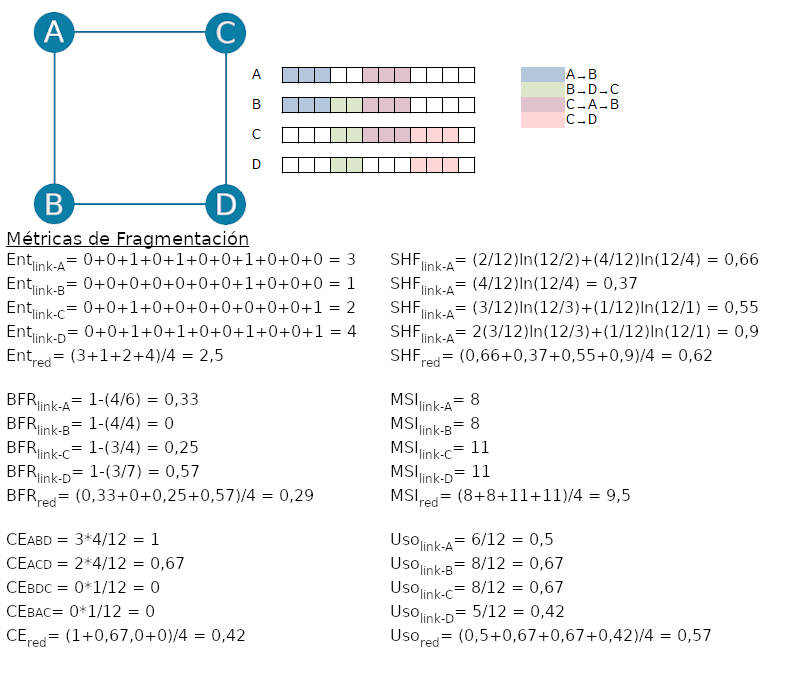
\includegraphics[width=1\textwidth]{capitulos/img/ejemploMetricasCompleto4.png}
    \caption{Ejemplo de métricas de fragmentación}
    \label{fig:ejemploMetricas}
\end{figure}

En la figura \ref{fig:ejemploMetricas} se puede ver un ejemplo de una topología con 4 conexiones activas, el estado de sus enlaces y el cálculo de cada una de las métricas de fragmentación explicadas anteriormente. 

\section{Obtención de datos para el entrenamiento}
Se utilizó un simulador de redes EON \cite{davalos2019spectrum} para la generación del conjunto de datos a ser utilizados para el entrenamiento de la red neuronal.

Para esto se utilizaron dos topologías de red: USNET y NSFNET, en donde por cada topología se realizaron 50 simulaciones con volumen de  tráfico variable en la misma simulación, para lograr que la cantidad de conexiones activas no permanezca constante durante la simulación.  La variación de tráfico usada fue la que se ve en la figura \ref{fig:traficos}-a, el proceso se realizó durante 1210 unidades de tiempo para cada simulación, generando un total de 121.000 registros.

Una vez generados los datos, los mismos fueron preprocesados, de forma a obtener los valores de la probabilidad de bloqueo que deseamos estimar.

El preprocesamiento consiste en el cálculo del índice de bloqueo en base a la ecuación \ref{eq:ecuacion_ib}, donde para un tiempo t, utilizando una ventana de 10 unidades de tiempo hacia delante, para cada instante podemos obtener una mirada hacia delante de posibles bloqueos, \(FSB_{i}\) es la sumatoria de \textit{FS} bloqueados en el tiempo \textit{i} y \(FSD_{i}\) es la sumatoria de \textit{FS} demandados en el tiempo \textit{i}.

\begin{equation} \label{eq:ecuacion_ib}
        PB_{t} = \frac{\sum_{i=t}^{t+T}FSB_{i}}{\sum_{i=t}^{t+T}FSD_{i}}
\end{equation}

Además, una vez separados los datos y debido a la diferencia de rangos de valores, los mismos son normalizados, usando la siguiente fórmula.
\begin{equation}
    n = x - \frac{train_{mean}}{train_{std}}
\end{equation}
Donde x es el valor que queremos normalizar, \(train_{mean}\) la media de valores y \(train_{std}\) es la desviación estándar. 

\begin{figure}
    \centering
    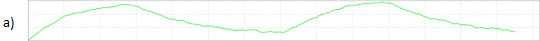
\includegraphics[width=1\textwidth]{capitulos/img/trafico_1_a.png}
    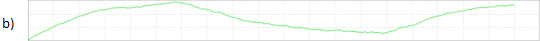
\includegraphics[width=1\textwidth]{capitulos/img/trafico_2_b.png}
    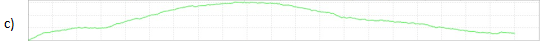
\includegraphics[width=1\textwidth]{capitulos/img/trafico_3_c.png}
    \caption{Volumen de tráfico variado utilizado}
    \label{fig:traficos}
\end{figure}

\section{Herramientas Utilizadas}

En esta sección se presentan las herramientas utilizadas para la implementación del método propuesto en este trabajo, seleccionadas luego de realizar numerosas ejecuciones de prueba para obtener los valores de los parámetros del modelo, asi como la prueba de concepto en sí.

Para todo el proceso de \textit{Machine Learning} se utilizó la plataforma de código abierto llamada \textit{\textbf{TensorFlow}} \cite{tensowFlow} en el lenguaje de programación \textit{\textbf{Python}}. En la creación y entrenamiento de redes neuronales se utilizó la API de alto nivel incluida en la plataforma \textit{\textbf{Tensorflow}} denominada \textit{\textbf{Keras}}, la cual permite la creación de modelos de aprendizaje automático de forma rápida y sencilla.

Elegimos Tensorflow como herramienta principal debido a que es una plataforma de código abierto orientado a \textit{Machine Learning}. Cuenta con un ecosistema completo de herramientas y librerías que facilitan la creación y desarrollo de aplicaciones de aprendizaje automático, además cuenta con una extensa y muy completa documentación.

\section{Modelado}

Para entrenar los datos recolectados se utilizó un modelo con una capa de entrada de 7 neuronas, dos capas ocultas densamente conectadas, cada una con 64 y 32 neuronas respectivamente, y una capa de salida que devuelve un único valor continuo.
Para todas las capas la función de activación utilizada fue la RELU (Ver sección 3.2.2).

\section{Entrenamiento}
Para el entrenamiento del modelo, se creó un conjunto de datos de entrenamiento utilizando el 70\% de los datos recolectados de forma aleatoria.  

El 20\% de los datos de entrenamiento se utilizó como el conjunto de validación. Una técnica utilizada en el procedimiento es el  llamado parada temprana o \textit{Early Stopping}, el cual mediante el monitoreo del rendimiento del entrenamiento nos permite detenernos una vez que el error de validación aumente de forma sostenida, de forma así evitar un sobre entrenamiento.

El modelo se entrena como máximo por 1000 épocas, el cual se detiene automáticamente cuando el valor del error de validación deja de mejorar. La figura \ref{fig:errorEpocas} muestra la evolución del error al pasar las épocas.

Los parámetros comparados son el error de entrenamiento o \textit{Train Error}, el cuál es el error obtenido durante la fase de entrenamiento del modelo y el error de validación o \textit{Val Error}, que se obtiene en la fase de validación.

Por cada época el \textit{Val Error} es comparado con el  \textit{Train Error},esto hasta que se determina que ya no existe mejora, sino que el error de validación se mantiene o aumenta su valor con respecto al punto de parada.


\begin{figure}[H]
    \centering
    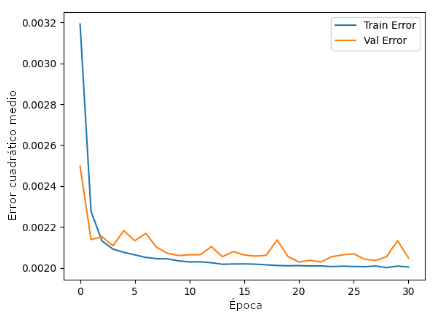
\includegraphics[width=9cm]{capitulos/img/graficoErrorEs.png}
    \caption{Evolución del error a través de épocas}
    \label{fig:errorEpocas}
\end{figure}

\section{Pruebas de predicción}
Para comprobar la efectividad de nuestro modelo se procedió a tomar el 30\% de datos restantes que no fueron incluidos en el entrenamiento y realizar predicciones, como ya conocemos el valor de la probabilidad de bloqueo que se busca predecir podemos calcular el error absoluto medio (MAE) y el error cuadrático medio (MSE). La tabla \ref{table:resultadosPrediccionTabla} muestra los resultados obtenidos, siendo éstos muy satisfactorios.

\begin{table}[H]
\centering
    \caption{Tabla de resultados en pruebas de predicción}
    \begin{tabular}{|l|l|}
        \hline
        MAE & 0.0239 \\ \hline
        MSE & 0.002  \\ \hline
    \end{tabular}
    \label{table:resultadosPrediccionTabla}
\end{table}
\newpage
\begin{figure}[H]
    \centering
    \begin{tabular}{@{}c@{}}
        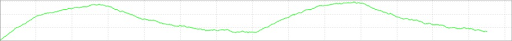
\includegraphics[width=1\textwidth]{capitulos/img/trafico_1.png}\\
        \small (a) Tráfico de volumen variable
    \end{tabular}
    \begin{tabular}{@{}c@{}}
        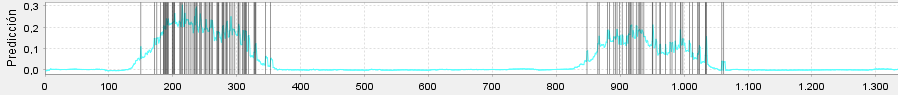
\includegraphics[width=1\textwidth]{capitulos/img/grafico_prediccion_usnet.PNG}\\
        \small (b) Gráfico de valores predichos por la red neuronal
    \end{tabular}
    \caption{Utilización de la red y predicciones}
    \label{fig:utilizacionPredicciones}
\end{figure}
En la Figura \ref{fig:utilizacionPredicciones} - a se observa la variación de la utilización de la red, al realizarse una simulación con volumen de tráfico variable sin realizar procesos de desfragmentación. En la parte b de la misma figura se observa la curva de valores predichos con las técnicas presentadas junto a los bloqueos dados en la misma simulación. Puede observarse cómo este valor acompaña la variación de la utilización de la red, y también toma valores más altos en periodos de tiempo en que la frecuencia de bloqueos se hace más alta. 

\chapter{ Pruebas y resultados obtenidos }
Las pruebas se realizaron sobre el simulador de redes elásticas ópticas desarrollado en \cite{davalos2019spectrum} con las topologías USNET y NSFNET, la generación de demandas se realiza de manera aleatoria, pero con variaciones de volumen de tráfico. En la figura \ref{fig:traficos} se pueden ver las curvas de rutas activas, siendo el eje \textit{x} el tiempo y el eje \textit{y} la cantidad de rutas activas, para lograr esto inicialmente la simulación inicia con 700 Erlangs y al llegar la utilización de la red a un valor máximo baja a 100 Erlangs, de esta forma conseguimos que la carga de la red no sea constante y podamos acercarnos a un escenario más real. Para el proceso de desfragmentación se utilizó el algoritmo genético propuesto en \cite{davalos2019spectrum}.

El proceso que seguimos para seleccionar el periodo de tiempo en el que el proceso de desfragmentación se ejecutará se puede ver en la figura \ref{fig:simuladorModelo}, donde las características son las citadas en el capítulo 4 sección 4.1, \textit{PB} es la probabilidad de bloqueo calculada por nuestro modelo entrenado, \(PB_{th}\) es el valor seleccionado como umbral para que el proceso de desfragmentación se dispare y \textit{DF} es el proceso de desfragmentación.  

\begin{figure}[h!]
    \centering
    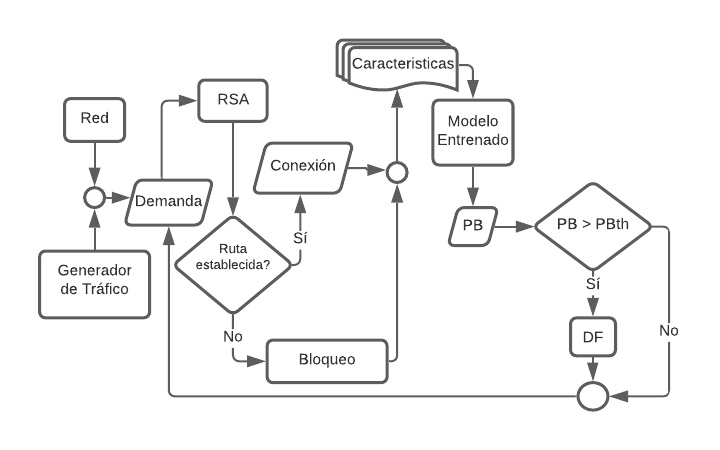
\includegraphics[width=1\textwidth]{capitulos/img/diagramaML6.png}
    \caption{Diagrama simulador / modelo entrenado}
    \label{fig:simuladorModelo}
\end{figure}

Para tener un punto de referencia nuestro modelo se compara con otros dos métodos conocidos:
\begin{itemize}[a)]
    \item Desfragmentación periódica por tiempo fijo: el cual consiste en desfragmentar la red cada cierta cantidad constante de unidades de tiempo.
    \item Desfragmentación por métricas de fragmentación: el cual consiste en desfragmentar cuando la red alcanza cierto valor de alguna métrica, en este caso de BFR.
\end{itemize}

Cada método tiene su propio parámetro encargado de disparar el proceso de desfragmentación y durante las pruebas se hace variar este parámetro hasta tres veces. 

Para elegir este valor tomamos como base la cantidad de desfragmentaciones que realiza el método por tiempo fijo y se buscan valores para los parámetros de los otros métodos de tal manera que ejecuten cantidades similares de desfragmentaciones, así logramos que la comparación se haga de la forma más justa posible.

Las simulaciones se realizaron con los tres métodos bajo las mismas condiciones de variaciones de distribuciones demandas y parámetros, para obtener mayor variación en los resultados este procedimiento se repitió 5 veces.

\section{Objetivos a optimizar}

Para la evaluación de los resultados, considerando dos objetivos globales, medidos al final de cada simulación:

\begin{enumerate}[Obj. 1)]
    \item \textbf{Cantidad de bloqueos(BL):} Suma de las demandas bloqueadas durante la simulación
    \item \textbf{Cantidad de reconfiguraciones(RC):} Número de conexiones reconfiguradas durante los procesos de desfragmentación realizadas durante la simulación. 
\end{enumerate}

Como se trata de dos objetivos a optimizar (BL y RC), buscando minimizar el valor de ambas, para la comparación de los resultados se consideraron dos métricas de desempeño para optimización multi-objetivo \cite{von2014survey}: 

\begin{itemize}
    \item \textbf{Número de soluciones en el Frente Pareto obtenido (SFP):} Para esta primera métrica, se busca determinar el método que contenga el mayor número de soluciones no dominadas que minimicen BL y RC, comparando al mismo tiempo las soluciones de nuestro método propuesto con las soluciones de los otros dos métodos. 
    
     \item \textbf{Cobertura Pareto(CP):} Como segundo método de comparación utilizamos una métrica binaria denominada “Cobertura”, la cual nos permite realizar la comparación de las soluciones óptimas de nuestro método propuesto con los demás métodos tomándolos de a pares.
 
 \begin{equation}
      C(A,B) = \frac{Soluciones\ de\ B\ dominadas\ por\ A}{Soluciones\ totales\ de\ B}  
 \end{equation}
    

\section{Análisis de los resultados}

Se puede observar en la Tabla \ref{tab:frentePareto} que de todas las instancias experimentales que se encuentran en el Frente Pareto, el método propuesto (MP) en este trabajo representa el 52.9\% de los puntos dentro del mismo, lo que indica que este método produce más soluciones no dominadas, indicando una mayor eficiencia en lo que respecta a la minimización de la cantidad de bloqueos y el número de reconfiguraciones en la red.

\begin{table}[h!]
    \centering
    \caption{Tabla de soluciones en el frente pareto}
    \begin{tabular}{|c|c|c|c|c|}
    \hline
    \multirow{2}{*}{\textbf{SIMULACIÓN}} & \multicolumn{4}{c|}{\textbf{Soluciones del Frente Pareto}}\\ \cline{2-5} 
         & \textbf{MP} & \textbf{Tiempo Fijo} & \textbf{BFR} & \textbf{Total}\\
    \hline
    NSFNET & \textbf{9} & 4 & 6 & 19\\
    USNET & \textbf{9} & 4 & 2 & 15\\
    \hline
    
    \end{tabular}
    \label{tab:frentePareto}
\end{table}

 En las figuras \ref{fig:paretoNSFNET} y \ref{fig:paretoUSNET} podemos observar los resultados para los tres diferentes tipos de tráfico, para el caso de la topología USNET (figura \ref{fig:paretoUSNET}), en el frente de soluciones óptimas se aprecia una predominancia del método propuesto en cuanto a cantidad de soluciones. Mientras que en el caso de la topología NSFNET  (figura \ref{fig:paretoNSFNET}), dicha predominancia se puede ver en dos de los tres tipos de tráfico.
 \newpage
 
 \begin{figure}[H]
    \centering
    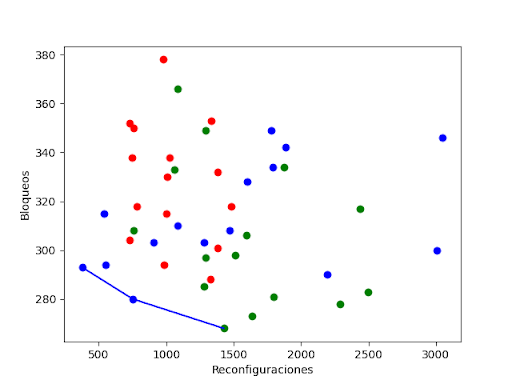
\includegraphics[width=0.9\textwidth]{capitulos/img/nsfnet_pareto_1.png}
    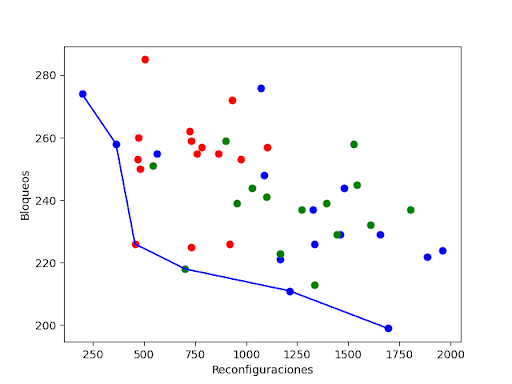
\includegraphics[width=0.9\textwidth]{capitulos/img/nsfnet_pareto_2.png}
    \caption{Gráfico de soluciones en el frente pareto para la topología NSFNET}
 \end{figure}

 \begin{figure}[H]\ContinuedFloat
    \centering
    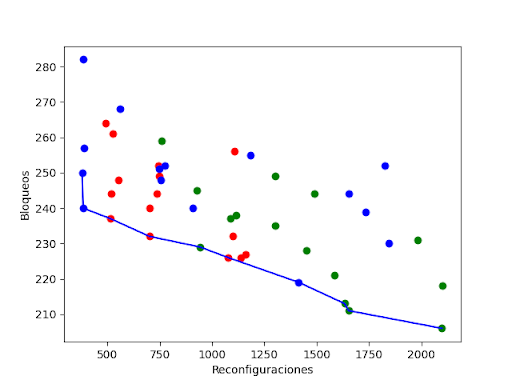
\includegraphics[width=0.9\textwidth]{capitulos/img/nsfnet_pareto_3.png}
    \caption{Gráfico de soluciones en el frente pareto para la topología NSFNET}
    \label{fig:paretoNSFNET}
 \end{figure}

 \begin{figure}[H]
    \centering
    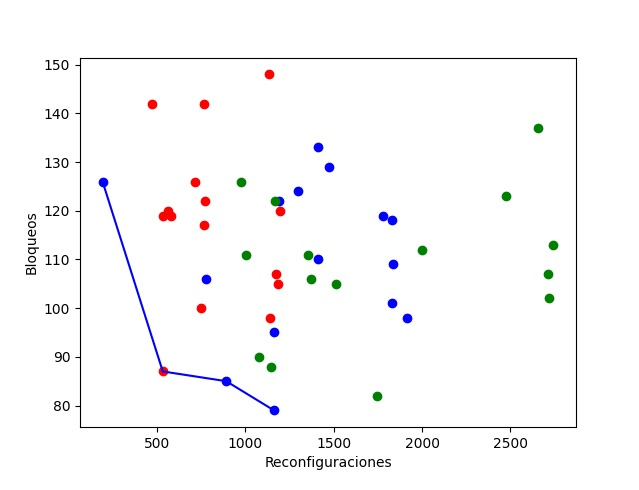
\includegraphics[width=0.9\textwidth]{capitulos/img/paretoUsnetSB.jpg}
    \caption{Gráfico de soluciones en el frente pareto para la topología USNET}
 \end{figure}
\begin{figure}[H] \ContinuedFloat
    \centering
    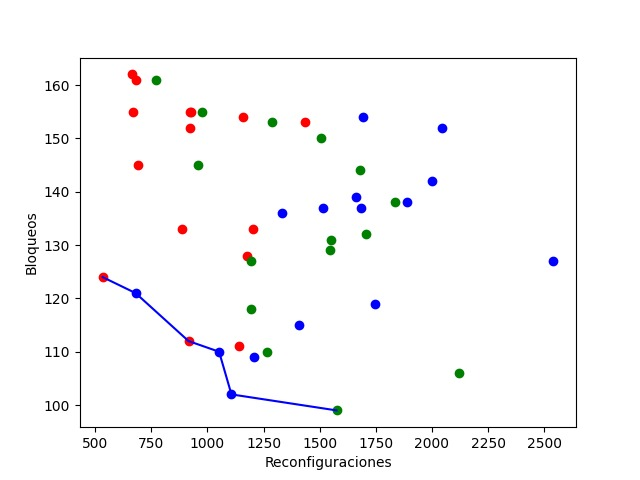
\includegraphics[width=0.9\textwidth]{capitulos/img/paretoUsnetSBSB.jpeg}
    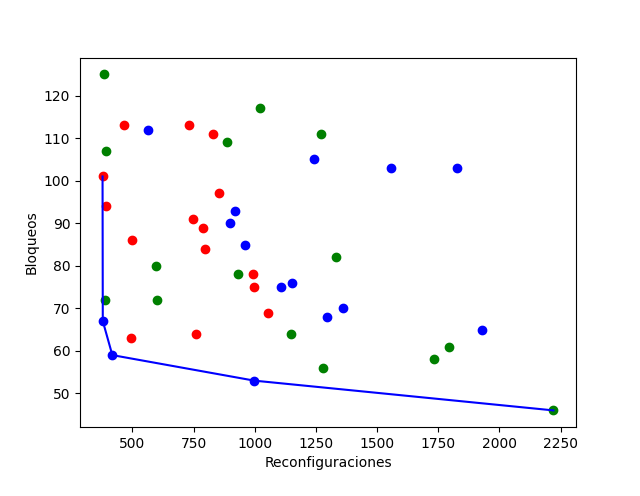
\includegraphics[width=0.9\textwidth]{capitulos/img/paretoUsnetSBS.png}
    \caption{Gráfico de soluciones en el frente pareto para la topología USNET}
    \label{fig:paretoUSNET}
\end{figure}
\newpage

En las tablas \ref{tab:frenteParetoUSNET} y \ref{tab:frenteParetoNSFNET} se presentan los resultados de la métrica CP, para los tres tipos de tráfico, donde \textit{MP} es el método propuesto, \textit{TF} el método por tiempos fijos y \textit{BFR} es el método por métricas. Se verifica que en un 67\% del total de comparaciones, incluidas las dos topologías, el método propuesto obtiene mayor cobertura en las soluciones óptimas.
  
\begin{table}[h!]
    \centering
    \caption{Tabla de cobertura para topología USNET}
    \begin{tabular}{|c|c|c|l|l|l|}
    \hline
    \multicolumn{6}{|c|}{USNET}
    \\ \cline{1-6}
    Tráfico & A & B & C(A,B) & C(B,A) & Conclusión \\
    \hline
4.2-a & MP & TF & 0,5 & 0,25 & \makecell{\textbf{A cubre a B en un 50\%} \\ \textbf{y es cubierto en un 25\%}} \\
4.2-a & MP & BFR & 1 & 0 & \makecell{\textbf{A cubre a B en un 100\%} \\ \textbf{y es cubierto en un 0\% }}\\
4.2-b & MP & TF & 0,67 & 0 & \makecell{\textbf{A cubre a B en un 67\%} \\ \textbf{y es cubierto en un 0\% }}\\
4.2-b & MP & BFR & 0,8 & 0 & \makecell{\textbf{A cubre a B en un 80\%} \\ \textbf{y es cubierto en un 0\% }}\\
4.2-c & MP & TF & 0,5 & 0,67 & \makecell{B cubre a A en un 67\% \\ y es cubierto en un 50\%} \\
4.2-c & MP & BFR & 0 & 0 & \makecell{No existe cobertura} \\
\hline
    \end{tabular}
    \label{tab:frenteParetoUSNET}
\end{table}

\begin{table}[h!]
    \centering
    \caption{Tabla de cobertura para topología NSFNET}
    \begin{tabular}{|c|c|c|l|l|l|}
    \hline
    \multicolumn{6}{|c|}{NSFNET}
    \\ \cline{1-6}
    Tráfico & A & B & C(A,B) & C(B,A) & Conclusión \\
    \hline
    
%1 & IA & Periódico & 0,25 & 0 & \makecell{\textbf{A es mejor que B porque lo cubre en} \\ \textbf{un 50\% y es cubierto en un 33\%}}\\
4.2-a & MP & TF & 0,25 & 0 & \makecell{\textbf{A cubre a B en un 25\%} \\ \textbf{y es cubierto en un 0\%}} \\
4.2-a & MP & BFR & 0,43 & 0 & \makecell{\textbf{A cubre a B en un 43\%} \\ \textbf{ y es cubierto en un 0\% }}\\
4.2-b & MP & TF & 0 & 0,29 & \makecell{B cubre a A en un 29\% \\ y es cubierto en un 0\%} \\
4.2-b & MP & BFR & 0,33 & 0,43 & \makecell{B cubre a A en un 43\% \\ y es cubierto en un 33\%} \\
4.2-c & MP & TF & 1 & 0 & \makecell{\textbf{A cubre a B en un 100\%} \\ \textbf{ y es cubierto en un 0\% }}\\
4.2-c & MP & BFR & 0,67 & 0 & \makecell{\textbf{A cubre a B en un 67\%} \\ \textbf{ y es cubierto en un 0\%}} \\
\hline
    \end{tabular}
    \label{tab:frenteParetoNSFNET}
\end{table}

\end{itemize}





\chapter{ Conclusiones y Trabajos Futuros }

En las redes ópticas elásticas, la constante asignación y liberación de recursos en forma dinámica puede dar lugar al problema conocido como "fragmentación del ancho de banda". Este problema es crítico ya que la presencia de bloques aislados de ancho de banda dentro del dominio del espectro deja a los mismos inutilizables ante futuras solicitudes de conexiones, debido a que los mismos no se encuentran alineados y contiguos,

Un enfoque utilizado para combatir la fragmentación son los procesos de desfragmentación, que consisten en el retiro y posterior re-ruteo de un sub-conjunto de conexiones existentes, con el objetivo de consolidar los espacios disponibles en grandes bloques contiguos y continuos que puedan ser utilizados para futuras solicitudes de conexiones.

El problema analizado en este trabajo es el de ¿Cuándo Reconfigurar?, es decir, buscar el momento adecuado para disparar el proceso de desfragmentación, ya que desfragmentaciones muy frecuentes o muy distantes en el tiempo pueden hacer que estos no sean muy eficientes.

Este trabajo presenta un enfoque con desfragmentación para tráfico dinámico de redes ópticas elásticas por medio de un disparador inteligente utilizando técnicas de \textit{Machine Learning}. En su implementación se utilizó un enfoque de aprendizaje supervisado, con un modelo de redes neuronales artificiales para la predicción de futuros bloqueos y utilizando algunas características para medir el estado de fragmentación de la red y el uso de la misma.

El método propuesto de disparo recibe el estado actual de la red o ``características'' para cada instante de tiempo, con estas características y el entrenamiento previo del modelo, obtenemos una predicción de la probabilidad de futuros bloqueos, para una ventana de 10 unidades de tiempo hacia delante.

Para evaluar la eficiencia del método propuesto de disparo se consideraron tres escenarios diferentes, con un volumen de tráfico variable, utilizando las topologías NSFNET y USNET. Los objetivos a optimizar fueron: 
\begin{itemize}
    \item La cantidad de bloqueos obtenidos (BL)
    \item La cantidad de reconfiguraciones al final de cada instancia de prueba (RC)
\end{itemize}

\section{Conclusiones Experimentales}
Se realizaron pruebas experimentales a fin de comparar nuestro método de disparo contra otros dos presentes en la literatura científica. El método de desfragmentanción periódica es una estrategia ampliamente utilizada, la cual consiste en realizar el proceso de desfragmentación cada cierto periodo fijo de tiempo y el disparo por medio de métricas, la cual considera en realizar el proceso de desfragmetación en base al valor actual de la métrica, para las pruebas de este método se utilizó la métrica de fragmentación BFR.

Para comparar los resultados obtenidos en relación a los objetivos citados anteriormente (BL y RC), se utilizaron dos métricas de desempeño para optimización multi-objetivo.

\begin{enumerate}
    \item Número de soluciones en el Frente Pareto (SFP).
    \item Cobertura Pareto (CP).
\end{enumerate}

Como resultado de la comparación de los métodos en base a los objetivos expuestos previamente, se concluye que el método propuesto es mejor ya que consigue en la mayoría de los escenarios mejores resultados,
minimizando los valores obtenidos para BL y RC. Considerando la métrica SFP se obtiene que constituye el 52.9\% de soluciones no dominadas y en el caso de CP se logró en un 67\% del total de comparaciones resultados favorables a nuestro método.

\section{Aportes}
Los aportes del presente trabajo son:
\begin{enumerate}[label=\arabic*)]
    \item Un análisis bibliográfico sobre el problema relacionado al periodo de tiempo en el que el proceso de desfragmentación será ejecutado.
    \item Una investigación y recopilación de métricas de fragmentación las cuales son utilizadas como características necesarias para la predicción de la probabilidad de bloqueo por parte del modelo entrenado.
    \item Como principal aporte se diseñó un algoritmo que realiza el preprocesamiento de datos, entrenamiento del modelo y predicción de probabilidades de bloqueo utilizando técnicas de \textit{Machine Learning}.
    \item Pruebas experimentales utilizando en conjunto un simulador de redes EON y el modelo entrenado a fin de evaluar la eficiencia de nuestro método propuesto. Se realizaron comparaciones contra otros dos mecanismos de disparo, disparo periódico en tiempos fijos y disparo basado en la métrica BFR, teniendo resultados favorables para nuestro método en relación a la minimización de la cantidad de bloqueos y reconfiguraciones.
\end{enumerate}

\section{Trabajos Futuros}
\begin{itemize}
    \item Aplicar el modelo de disparo inteligente del proceso de desfragmentación propuesto en este trabajo a redes ópticas elásticas que utilizan otras tecnologías o técnicas, como las redes EON con multiplexación por división de espacios o \textit{Space División Multiplexing} (SDM).
    
    EL SDM es utilizado en redes con múltiples núcleos, por lo que sería interesante realizar un análisis de la eficiencia del modelo en este tipo de redes.
    
    \item Proponer algoritmos de disparo del proceso de desfragmentación utilizando métodos estadísticos, tal como la regresión logística binaria (RLB), la cual se utiliza cuando se desea conocer la relación entre una variable dependiente binaria y una o más variables independientes o explicativas, las cuales pueden ser cuantitativas y/o cualitativas.
    
    El objetivo de la RLB es obtener una estimación ajustada de la probabilidad de ocurrencia de un evento a partir de una o más variables independientes.
    
    \item Otro enfoque posible es utilizar programación genética, el cual consiste en una metodología basada en algoritmos evolutivos e inspirada en la evolución biológica para desarrollar programas que realicen ciertas tareas, por ejemplo, realizar disparo del proceso de desfragmentación en el mejor momento.
    
    Es una técnica de aprendizaje automático utilizada para optimizar una población de programas de acuerdo a una función de ajuste o \textit{fitness function} que evalúala capacidad de cada programa de realizar la tarea.
\end{itemize}
	
	
	


\appendix   % inician los apendices de tu tesis
% los cap'itulos que incluyas a partir de aqu'i aparecen
% como ap'endices
\include{./anexo-1}
% estos comandos generan la bilbiograf'ia

\printbibliography

\end{document}
